\documentclass{article}

\usepackage[utf8]{inputenc}
\usepackage{natbib}

\usepackage{graphicx}
\usepackage{subcaption}
\usepackage[section]{placeins}
\usepackage{fullpage}
\usepackage[affil-it]{authblk}
\usepackage{todonotes}

\usepackage{amsmath}
\usepackage{amssymb}
\usepackage{bbold}
\usepackage{mathrsfs}
\usepackage{bm}

\usepackage{algorithm}
\usepackage[noend]{algorithmic} 

\DeclareMathOperator{\Tr}{Tr}
\DeclareMathOperator{\cst}{cst}
\DeclareMathOperator{\Gram}{Gram}
\DeclareMathOperator{\R}{\mathbb{R}}
\DeclareMathOperator{\1}{\mathbb{1}}
\DeclareMathOperator{\E}{\mathbf{E}}
\DeclareMathOperator{\Y}{\mathcal{Y}}
\DeclareMathOperator*{\argmax}{arg\,max}
\DeclareMathOperator*{\argmin}{arg\,min}
\DeclareMathOperator{\dom}{Dom}

\title{Stochastic Dual Coordinate Ascent \\ for \\ Conditional Random Fields}
\author{R\'emi LE PRIOL}
\affil{Montreal Institute of Learning Algorithms}
\date{\today}

\begin{document}

\maketitle

\section*{Introduction}
In his paper \cite{shalev-shwartz_accelerated_2013-1}, Shalev-Shwartz describes and analyzes the Stochastic Dual Coordinate Ascent algorithm (SDCA) to solve empirical risk minimization problems.
SDCA updates coordinates of the dual variable, one at a time or block by block, so as to raise the dual score.
He proves that SDCA has a linear convergence rate for these problems when the loss-functions are smooth.

We apply SDCA on the $l^2$ regularized negative log-likelihood minimization.
Given n sample $x_i \in \mathcal X$ and their labels $y_i \in \Y$, the problem we aim to solve has the form:
\begin{equation}
	\label{max likelihood}
	 \min_{w \in \R^d} \frac{\lambda}{2}\|w\|^2 - \frac{1}{n}   \sum_{i=1}^{n} \log(p(y_i|x_i; w))
\end{equation}
The minimization takes place over the weight vector w parametrizing the conditional probability of y given x. 
  
First we focus on problems where the number of classes $|\Y|$ is small, such as multinomial logistic regression.
For such problems, SDCA's application is straightforward from \cite{shalev-shwartz_accelerated_2013-1}.
We propose a Non-Uniform adaptive Sampling scheme (NUS) to improve the convergence speed.
We test this approach on synthetic gaussian mixtures and on the covertype dataset introduced in \cite{blackard_comparative_1999}.
 
Then we apply SDCA to structured prediction.
In structured prediction, each class or label is a structured object.
This problem is notoriously hard because the set of labels $\Y$ is exponentially large in the size of x.
For instance, if $x$ is a sequence of images of letters, then $\Y$ is the set of sequences of  letters with the same length as $x$.
In the Optical Character Recognition dataset (OCR, \cite{taskar_max-margin_2004}), the mean word length is 7.5.
There exist $26^7 \sim 10^{10}$ lower case strings of length 7.
This is too large to be explored naively.

Our main contribution is to adapt SDCA to exploit the structure in the labels.
In the Conditional Random Fields model (CRF, \cite{lafferty_conditional_2001} ), the conditional distribution $p(y|x ; w)$ has a structure.
This structure is described by an undirected graphical model (a.k.a. Markov Random Fields). 
The dual problem's natural variables are the conditional joint probabilities $p(y|x_i ; w)$.
We have to manipulate this joint for every data point, while not even one of them fits in memory.
We adapt SDCA by operating on marginal probabilities instead of the joints.
We transpose the non-uniform sampling scheme to this version of SDCA.

SDCA is a good candidate algorithm to train CRF.
It has a linear convergence rate.
It performs an exact line search for a limited cost.
We apply SDCA on the OCR dataset.
This work is still in progress.
We provide preliminary results.

\clearpage
\tableofcontents

\section{Background}
The problem \ref{max likelihood} has a long running history in the machine learning community.
A number of approaches have been tried.
The main difficulty is the ever-increasing number of samples n.
In 2001, \cite{lafferty_conditional_2001} described the CRF model and proposed an iterative scaling approach.
That was not as efficient as the generic deterministic algorithm : limited-memory memory quasi-Newton (L-BFGS, \cite{wallach_efficient_2002}, \cite{sha_shallow_2003}).
Deterministic algorithms require performing some computation for each of the n data points at each step.
This is not tractable for very large n.
Researchers have tried to apply stochastic methods such as the stochastic gradient descent (\cite{vishwanathan_accelerated_2006}, \cite{finkel_efficient_2008}).
These methods have a sub-linear convergence rate.
They take $O(1/\epsilon)$ iterations to reach precision $\epsilon$.
This is much larger than the $O(\log(1/\epsilon))$ iterations required by deterministic methods (this is called a linear rate).

\paragraph{Variance Reduction.}
This is where the variance reduction methods come into play.
These methods achieve both a linear convergence rate, and a cheap update cost (independent of n).
There is a trade-off though.
They also require a memory  $O(n)$.
Thanks to this memory these methods avoid staying on the surface of the variance ball, as in the stochastic gradient descent.
They get an update whose variance vanish as we get closer from the optimum.
The family of variance reduction  include : 
\begin{itemize}
	\item	 Exponentiated Gradient in 2008 \cite{collins_exponentiated_2008}, developed primarily for structured prediction.
	\item Stochastic Average Gradient (SAG) in 2012 \cite{roux_stochastic_2012}
	\item SDCA in 2013
	\item Stochastic Variance Reduced Gradient (SVRG) in 2014 \cite{johnson_accelerating_2013} which coined the term "variance reduction"
	\item SAGA in 2014 \cite{defazio_saga:_2014} which showed that all these methods have the same structure.  
\end{itemize}

\paragraph{Application to CRF.}
The exponentiated gradient was meant to train CRF models.
Its linear convergence is guaranteed only on the dual objective.
Its empirical performance is very inconsistant, sometimes state of the art, sometimes poorer than L-BFGS or the stochastic gradient (see figure 1 in \cite{schmidt_non-uniform_2015}). 
In 2014 \cite{schmidt_non-uniform_2015}, Schmidt adapted SAG to train CRF models.
He got state of the art results on a number of sequence datasets, totally outperforming the exponentiated gradient and other competitors.
Our contribution is in the direct lineage of these two works.
SDCA is very similar to the Exponentiated Gradient.
Both operates in the dual, but SDCA's linear convergence rate is  guaranteed on the duality gap.
This is theoretically stronger than the exponentiated gradient.
That makes SDCA closer from SAG in terms of theoretical guarantee.

The strong theoretical advantage of SDCA is its line search.
We can perform an exact line search for a very limited cost.
This is in contrast with SAG and the exponentiated gradient where the line search is very expensive.

\paragraph{Non-Uniform Sampling}
Schmidt improved SAG with a non-uniform sampling scheme.
A variety of non-uniform sampling schemes have been proposed for SDCA, such as \cite{csiba_stochastic_2015} which applies to binary classification.
We propose a new approach inspired by \cite{osokin_minding_2016} to improve the Block Coordinate Franck Wolfe algorithm from \cite{lacoste-julien_block-coordinate_2012}.
We sample proportionally to estimates of individual duality gaps.
The assumption is that if a point has a high duality gap, we will decrease more efficiently  the overall duality gap by moving that point. 

\paragraph{Convergence rates.}
Below we reproduce a table from \cite{schmidt_non-uniform_2015} stating the convergence rates of different methods for training CRFs.
It includes the fastest known rates for deterministic algorithms (like L-BFGS), stochastic algorithms (like [averaged] stochastic gradient), online exponentiated gradient, and SAG.
We append SDCA to this list.
We denote $L$ the Lipschitz constant of the gradient of the objective, and $m$ the strong-convexity constant .
We have $\lambda \leq m \leq L$.
We call $\sigma^2$ a bound on the variance of the gradients.\\
\begin{center}
\begin{tabular}{llc}
Deterministic & $O(n\sqrt{\frac{L}{m}}\log(1/\epsilon))$ & (primal)\\
Online EG & $O((n + \frac{L}{\lambda})\log(1/\epsilon))$ & (dual)\\
Stochastic & $O(\frac{\sigma^2}{m \epsilon}+\sqrt{\frac{L}{m \epsilon}})$ & (primal)\\
SAG & $O((n + \frac{L}{m})\log(1/\epsilon))$ & (primal) \\
SDCA & $O( (n + \min( \frac{L}{\lambda}, \sqrt{\frac{n L}{\lambda}}) ) \log(1/\epsilon) )$ & (duality gap)
\end{tabular}
\end{center}
Compared to SAG, SDCA suffer a dependency on the regularization parameter $\lambda$ instead of $m$.
It means that SAG is adaptative to  hidden strong-convexity, but not SDCA.
For large values of $\lambda$, the problem is very-strongly convex, and rather well  conditioned $L/m \leq L/\lambda \leq n$.
Then SAG has the best convergence rate.
On the other hand, if $\lambda$ is very small, SDCA may outperform SAG.
In between these extremes lies the typical value $\lambda=1/n$.
For such a value, if $m$ is close to $\lambda$, the outcome is uncertain.

\section{Multinomial Logistic Regression}

\subsection{Linear Models}

We consider the classical supervised learning setting.
We observe n data points $x_i \in \mathcal{X}$, with their labels $y_i\in \Y_i:= \{1,..,K\}$, for $i \in {1,..,n}$.
We index $\Y$ with i in order to be consistent with the structured part where the label space $\Y$ depends on the input $x_i$.
Similarly, we will index with i every function  whose domain of definition depend on the sample i.
We assume that the pairs $(x_i, y_i)$ are sampled independently and are identically distributed (i.i.d hypothesis).
Given a new vector $x$, we want to predict the corresponding label $y$. 
To do so, we first estimate a probability distribution over the classes $p(y|x ; w)$.
$w$ are the \textbf{w}eights that parametrize this distribution. 
The predicted label is then defined as a mode of this distribution : $\hat y = h_w(x) \in \argmax_y p(y| x ; w)$.

\paragraph{Features.}
We have no assumption on the space $\mathcal X$ but we have access to a feature extractor $F:\mathcal X \times \mathcal Y \rightarrow \R^d$.
These features can be either pre-trained or handcrafted.
For each couple data point - label, we get features as a vector of dimension $d$.

\paragraph{Linear Assumption.}
We assume that the score of a label is given as a linear function of its feature.
A consequence is that we have as many weights vas we have  features.
$w$ has dimension $d$.
We apply a softmax on these scores to get a probability vector. 
\begin{equation}
	\label{primal probability}
	p(y | x ; w) := \frac{\exp(w^TF(x, y))}{\sum_{y' \in \mathcal{Y}} \exp(w^TF(x, y'))}
\end{equation}

When there are few classes ($K \leq \sim 10^3$), the features we use are a block encoding of the class.
This is what is commonly called \textbf{multinomial logistic regression}.
If the $x_i$ are vectors of dimension $d'$, we set $d:=Kd'$. The feature vector $F(x, y)$ has a copy of $x$ on its $y$-th block of size $d'$, and zeros everywhere else.
In terms of linear model, this is the same as having one weight vector $w_y$ per class, so that $w^TF(x, y) = w_y^Tx$.
For the sake of comparison, this is like a shallow neural network with no hidden layer.
The input layer is of size $d'$.
The output layer of size K.
The weight matrix W of size $K \times d'$ is the vertical concatenation of the $w_y$.
We apply a softmax on the output layer.

\begin{figure}[ht]
	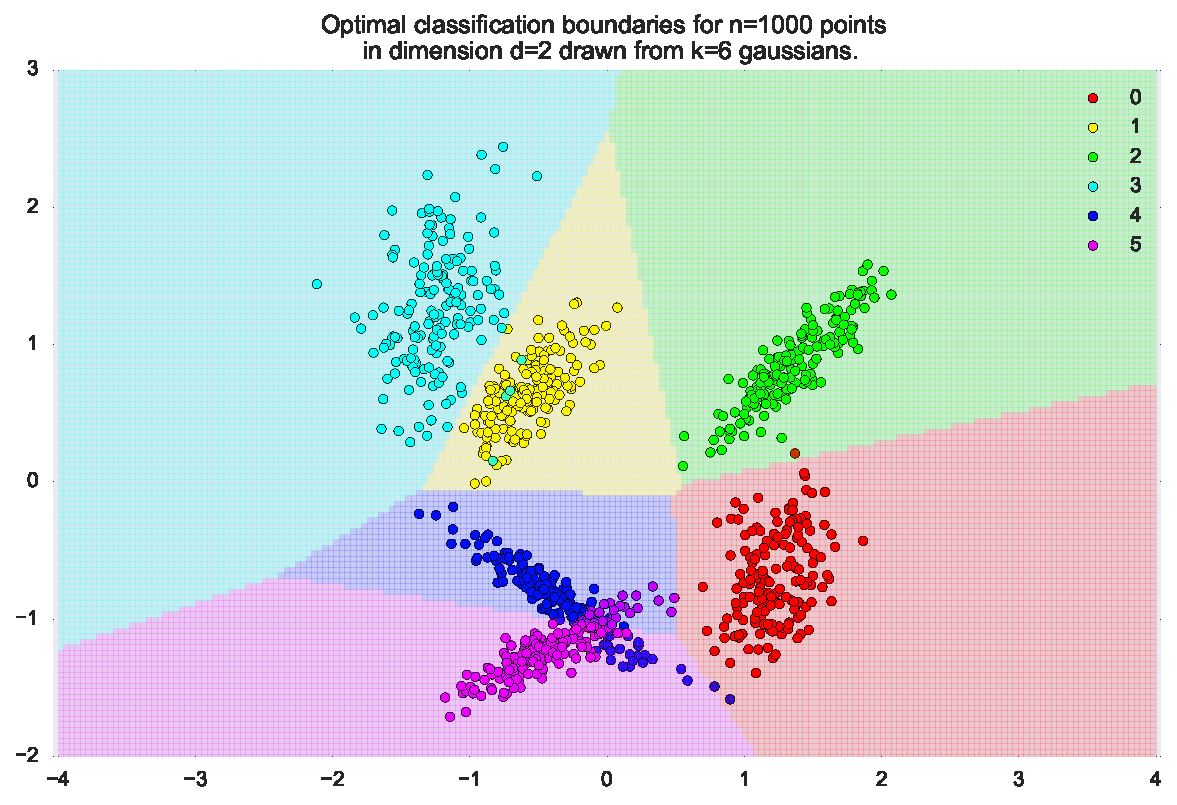
\includegraphics[width=\textwidth]{images/linear_classification.pdf}
	\caption{Optimal decision areas for the multinomial logistic regression.
	The data points are drawn from a balanced gaussian mixture in dimension 2.
	We set the bias constant to 1 and plot only the plan z=1.
	Each colour correspond to a class predicted by a linear model fitted on these points.}
	\label{linear boundaries}
\end{figure}

It should be noted that in general $d'$ includes a bias dimension.
The last coordinate of each x is set to 1 (or another constant).
The effective dimension where the x lives is $d'-1$.
With such models, we get polygonal classification boundaries in the effective space $\mathcal X = \R^{d'-1}$.
This is shown in figure \ref{linear boundaries} for $d'=3$, where we plot the plan $z=1$.
In the full space $\R^{d'}$, the decision areas are conic shapes centred on the origin.


 \subsection{Maximum Likelihood}

We want to fit our linear model to the observed samples $(x_i, y_i)$.
This means minimizing an empirical loss:
\begin{equation*}
	\min_w \sum_{y=1}^K \mathcal L (h_w(x_i),y_i)
\end{equation*}
where $\mathcal L: \Y \times \Y \rightarrow \R_+$ is a loss between labels.
A typical example is the 0-1 loss $\mathcal L(y, y') : = \1_{y=y'}$.
Unfortunately, this problem is very hard.
Since the loss is defined on a discrete space, there is no notion of continuity, even less so differentiability.
We are left with exhaustive search approaches which are intractable.
Hence the choice to consider the distribution probability $p( . | x ; w) \in \Delta_K$, where $\Delta_K$ denotes the simplex of dimension K.
We replace the discrete set $\Y$ by the continuous space $\Delta_K$.
We can define continuous or differentiable functions over this space, and get a tractable optimization problem.
 
We want our model to give the maximum probability to the observed pairs $(x_i, y_i)$.
The weights vector maximizing this probability is called maximum likelihood estimator.
Using the independence of the samples, and going to the log space, we formulate this as a sum of negative log-likelihood minimization problem.
To avoid overfitting, we regularize the problem by penalizing the $l^2$ norm of the weights.
We note $\lambda$ the regularization parameter. The primal objective to minimize is:
\begin{equation*}
\mathscr P(w) = \frac{\lambda}{2}\|w\|^2 - \frac{1}{n}   \sum_{i=1}^{n} \log(p(y_i|x_i; w))	
\end{equation*}
Using the linear assumption, we expand the log-likelihood:
\begin{equation*}
	\min_{w\in\R^d} \frac{\lambda}{2}\|w\|^2 + \frac{1}{n}   \sum_{i=1}^{n}  \log \big (\sum_y e^{w^TF(x_i, y)} \big ) - w^TF(x_i, y_i)	
\end{equation*}
To write this in a more compact way, we define the corrected features $\psi_i(y)$ of a class y for the sample i as the difference between the ground truth features and the features of $(x_i, y)$.
\begin{equation*}
	\psi_i(y)) := F(x_i, y_i) - F(x_i, y)
\end{equation*}
We can then remove the linear term from the objective:
\begin{equation*}
	\min_{w\in\R^d} \frac{\lambda}{2}\|w\|^2 + \frac{1}{n}   \sum_{i=1}^{n}  \log \big (\sum_y e^{- w^T\psi_i(y)} \big )
\end{equation*}
We can write this problem in a more vectorial form.
Denote the log-partition function (the log-sum-exp) $\phi(z) = \log \big(\sum_{y=1}^K \exp(z_y)\big)$. 
Denote $A_i$ the $d \times K$ matrix whose columns are the $\psi_i(y)$ for $y \in \Y_i$.
From now on we will refer to the following formulation as \textit{primal problem}.
\begin{equation}
	\label{primal problem}
	\min_{w\in\R^d}  \frac{\lambda}{2}\|w\|^2 + \frac{1}{n}   \sum_{i=1}^{n} \phi_i(-A_i^Tw)
\end{equation} 

\paragraph{Convexity.}
Let's show that this is a convex problem in w.
The $l^2$ penalty is of course convex.
The log-sum-exp is a convex function -- it is also smooth with constant $0.5$.
One can verify that it's Hessian is a semi-definite positive matrix.
We apply this convex function to a linear transformation of w.
Hence the convexity.
The $l^2$ regularization guarantees that the function we are optimizing is at least $\lambda$ strongly convex. 


\paragraph{Gradients.}
Let's notice that the gradient of the log-partition function evaluated on the score vector $-A_i^Tw$ is the conditional probability vector of the classes given x, as defined by the softmax function.
\begin{equation}
	\nabla \phi_i(-A_i^Tw) = (p(y | x_i ; w))_{y \in \Y_i}
\end{equation}
The gradient with respect to w of the full right hand term in (\ref{primal problem}) is the opposite of the expectation of the corrected features according to these probabilities.
\begin{equation}
	\label{primal gradient}
	\nabla_w (\phi_i(-A_i^Tw)) = - \E_{y \sim p(. | x_i ; w)} [\psi_i(y)]
\end{equation}
This will prove useful in the following.

\subsection{Dual Formulation}

As any convex problem, the maximum-likelihood admits dual formulations.
In this case, as the problem is unconstrained, we use Fenchel duality theorem to get a dual formulation.

\subsubsection*{Derivation}

We write $R(w) :=  \frac{\lambda}{2}\|w\|^2$ the convex regularization function. The primal problem becomes:
\begin{equation*}
	\min_{w \in \R^d}  R(w) + \frac{1}{n} \sum_{i=1}^n \phi_i(- A_i^T w)
\end{equation*}
We note $R^*$ and $\phi_i^*$ the convex conjugates (aka Fenchel dual functions) of $R$ and $\phi_i$ respectively.
The Fenchel dual associated to this problem is derived as follows :
\begin{align*}
	 \min_w \ R(w) + \frac{1}{n} \sum_i \phi_i(- A_i^T w) & = \min_w \ \max_{z\in \dom g^*} z^Tw - R^*(z) + \frac{1}{n} \sum_i \max_{\alpha_i \in \dom \phi_i^*} \alpha_i^T (-A_i^T w) - \phi_i^*(\alpha_i) \\
	 	& \geq \max_{z, \alpha} \  \min_w w^T(z - \frac{1}{n} \sum_i A_i \alpha_i) - R^*(z) - \frac{1}{n} \sum_i \phi_i^*(\alpha_i) \\
		& =  \max_{\alpha} \   - R^*(\frac{1}{n} \sum_i A_i \alpha_i) + \frac{1}{n} \sum_i -\phi_i^*(\alpha_i) \quad \textrm{if} \quad z= \frac{1}{n} \sum_i A_i \alpha_i \quad , -\infty \textrm{ otherwise.}\\
\end{align*}
When $R$ is the $l^2$ regularization, the convex conjugate is $R^*: z \mapsto \frac{1}{2\lambda}\|z\|^2$, with domain $\R^d$.
The convex conjugate of the log-sum-exp is the negative entropy. 
Its domain is $\Delta_i$ the simplex of dimension $K$.
\begin{equation}
	-\phi_i^*(\alpha_i) = H_i(\alpha_i) := - \sum_{y \in \Y_i} \alpha_i(y) \log(\alpha_i(y))
\end{equation}
Finally we get the dual problem of (\ref{primal problem}) in a closed form:
\begin{equation*}
	\max_{\alpha | \forall i, \alpha_i \in \Delta_i} \mathscr{D}(\alpha) = -\frac{1}{2\lambda} \| \frac{1}{n} \sum_i A_i \alpha_i \|^2 + \frac{1}{n} \sum_{i=1}^n H_i(\alpha_i)
\end{equation*}
The vector $\alpha$ has length $n\times K$.
Each of its n blocks live in the simplex.
The block $\alpha_i$ should be interpreted as a probability density on the labels for sample i.

\subsubsection*{Optimality Condition}
For this problem, \textbf{strong duality holds}.
The inequality in the derivation above is an equality.
This is true by the Fenchel Duality theorem because the $l^2$ regularization is defined on the whole space $\R^d$ and the log-sum-exp functions are continuous on their whole space as well.

The primal problem is strongly convex, so there is only one minimum.
Similarly, the dual problem is strongly concave, so there is only one maximum.
We consider the global optimum $(w^*,z^*,\alpha^*)$.
$(w^*,z^*)$ should be dual variables for the convex conjugates $(g, g^*)$.
\begin{equation*}
	g(w^*) + g^*(z^*) - \langle w^*, z^* \rangle = \frac{\lambda}{2} \| w^* - \frac{1}{\lambda} z^* \|^2 = 0
\end{equation*}
Hence the optimality condition:
\begin{equation*}
	w^* = 	\frac{1}{\lambda} z^* =  \frac{1}{\lambda n} \sum_i A_i \alpha_i^*
\end{equation*}
Consequently, we define the dual weights, or primal parameter associated to $\alpha$, written with a bold $\bm w$.
\begin{equation}
	\label{dual to primal}
	\bm w(\alpha) =   \frac{1}{\lambda n} \sum_i A_i \alpha_i
\end{equation}
These dual weights appear naturally in the dual problem. We use them to write the canonical expression of the dual problem.
\begin{equation}
	\label{dual problem}
	\max_{\alpha | \forall i, \alpha_i \in \Delta_i} -\frac{\lambda}{2} \| \bm w(\alpha) \|^2 + \frac{1}{n} \sum_{i=1}^n H_i(\alpha_i)
\end{equation}

Formula \ref{dual to primal} can be written in a number of ways, each time outlining some property.
We write A the horizontal concatenation of the $A_i$.
It is a matrix of size $d \times n\ K$.
\begin{align}
	\bm w(\alpha) & = \frac{1}{\lambda n} A \alpha \label{linearity} \\
	 & = \frac{1}{\lambda} \E_{i} [ \E_{y \sim \alpha_i} [\psi_i(y)]] \label{corrected features centroid} \\
	 & =   \frac{1}{\lambda} \E_{i} [F(x_i, y_i)] - \frac{1}{\lambda} \E_{i} [ \E_{y \sim \alpha_i} [F(x_i, y)]]
	 \label{centroid difference}
\end{align}
The expectations over i assume that i is a uniform random variable taking its values between 1 and n. 
Equation \ref{linearity} highlights the linearity in $\alpha$. Equation \ref{corrected features centroid} shows that this the centroid of the corrected features. Equation \ref{centroid difference} shows that this is the difference between the empirical feature centroid, and the centroids defined by $\alpha$.

We can also derive the primal problem from the dual problem.
We then get another optimality condition $\bm \alpha(w^*) = \alpha^*$.
$\bm \alpha(w)$ with a bold $\bm \alpha$ is the probability density on the training set defined by the weights w (equation \ref{primal probability}).
\begin{equation}
	\label{primal to dual}
	\forall i, \bm \alpha_i(w) = \nabla\phi_i(-A_i^Tw) = p(.|x_i; w) \propto \exp(-w^T \psi_i(.))
\end{equation}

\subsubsection*{Interpretation}
The primal problem is a regularized maximization of the likelihood of w. 
In the dual problem \ref{dual problem}, we control directly the probabilities given to each class on the training samples.
There are two conflicting terms.
The left hand one is the opposite of the squared distance between the centroid of the ground truth features and the centroids predicted by the dual model.
It is maximal for the empirical distribution.
The second term aims at maximizing the entropy of this distribution.
It pushes the $\alpha_i$ towards a more uniform distribution.
Thus the role of the terms is inverted compared to the primal problem : the data fitting term is the squared euclidean distance, and the regularization term is the entropy.

\paragraph{Naming :} 
We call \textit{primal model}, the one where we are given \textit{primal weights} $w$, from which we deduce \textit{primal probabilities} $\bm \alpha_i(w)$.
We call \textit{dual model}, the one where we are given \textit{dual probabilities} $\alpha_i$, from which we deduce \textit{dual weights} $\bm w(\alpha)$ as the centroid of the corrected feature vectors.
The optimality conditions tell us that at the optimum, these two models are equal.
$\alpha^*$ is a fixed point for $\bm \alpha \circ \bm w$.
$w^*$ is a fixed point for $\bm w \circ \bm \alpha$.
The optimization can be seen as a back and forth between the primal variable and the dual variable to find these fixed points.

%%%%%%%%%%%%%
\subsection{Duality Gaps}

The duality gap $g(w,\alpha)$ is the difference between the value  of the primal problem evaluated in $w$, and the value of the dual problem evaluated in $\alpha$.
\begin{equation*}
	g(w,\alpha) := \mathscr P(w) - \mathscr D(\alpha)
\end{equation*}
It is interesting to look at the duality gap for both the primal model and the dual model, i.e. the duality gap between the primal weights and the primal probability, and the duality gap between the dual weights and the dual probability.

\paragraph{Primal model:}
We inject the expression of $\bm \alpha_i(w)$ in the entropy to find the formula:
\begin{equation}
	\label{primal duality gap}
	g(w,\bm \alpha(w)) = \frac{\lambda}{2} \|w- \bm w(\bm \alpha(w))\|^2
\end{equation}
This formula involves $\bm w(\bm \alpha(w))$.
This is what the dual model created by the primal probabilities think the weights should be. 
In fact, using equation \ref{primal gradient} and \ref{dual to primal}, we can express the gradient of the primal objective 	as :
\begin{align*}
	\nabla \mathscr P(w) 
	& = \lambda w + \frac{1}{n} \sum_i \nabla_w(\phi_i(-A_i^Tw)) \\
	& = \lambda \bigg [ w - \frac{1}{\lambda n} \sum_i \E_{y \sim p(. | x ; w)} [\psi_i(y)] \bigg ] \\
	& = \lambda [ w - \bm w(\bm \alpha(w))]
\end{align*}
This means that the squared norm of the batch gradient is proportional to a duality gap.
\begin{equation}
	g(w,\bm \alpha(w)) = \frac{1}{2 \lambda} \|\nabla \mathscr P(w)\|^2
\end{equation}
In SAG, (see \cite{schmidt_non-uniform_2015}), Schmidt et al. use a biased estimator of the gradient as a descent direction.
They also use the norm of this estimator as a certificate to decide when to stop.
The justification is that since the gradient converges toward zero, the estimator converges toward zero as well.
If the objective is m-strongly convex there is also the bound:
\begin{equation*}
	\mathscr P (w) - \mathscr P(w^*) \leq \frac{1}{2 m}\|\nabla \mathscr P (w)\|^2
\end{equation*}
since the objective is at least $\lambda$-strongly convex we retrieve that the duality gap dominates the primal sub-optimality.
They are actually using an estimator of the duality gap as a certificate to decide when to stop.
For the cost of a another epoch, they could have the exact duality gap certificate.

\paragraph{Dual model:}
The gap for the dual model is naturally expressed as a sum of Fenchel duality gaps between the convex conjugates $\phi_i$ and $-H_i$. 
\begin{align*}
	g(\bm w(\alpha),\alpha) 
	& = \frac{1}{n} \sum_i \big [ \phi_i(-A_i^T \bm w(\alpha)) - H_i(\alpha_i) \big ] + \lambda \|\bm w(\alpha)\|^2 \\
	& =  \frac{1}{n} \sum_i \big [ \phi_i(-A_i^T \bm w(\alpha)) - H_i(\alpha_i) - \langle \alpha_i,  -A_I^T \bm w(\alpha) \rangle \big ]
\end{align*}
Each of the term in the sum above is positive.
They can be thought of as the duality gaps associated to each data point for the dual model.
We call them \textit{individual duality gaps}.
In particular, we have $\log(\alpha_i(w)) = -A_i^Tw - \phi_i(-A_i^Tw) \1$. Since $\alpha_i$ sums to one, we can inject this expression in the scalar product. We then get that each of the Fenchel duality gaps is also equal to the Kullback-Leibler divergence between the dual probability and the primal probability defined by the dual weights $\bm w(\alpha)$.
\begin{equation}
	\label{dual duality gaps}
	g(\bm w(\alpha),\alpha) = \frac{1}{n} \sum_i D_{KL} (\alpha_i || \bm \alpha_i(\bm w(\alpha))
\end{equation}
Once again, we observe a loop. Starting from the dual model, we define a primal which in turn defines a dual model.
\textit{Remark:} Performing SDCA with a step-size $\gamma=1$ gives the update formula $\alpha_i^+ = \bm \alpha_i(\bm w(\alpha))$, i.e. $ D(\alpha_i^+ || \bm \alpha_i(\bm w(\alpha)) )=0$. (See next section).

%%%%%%%%%%%%%%%%%
\subsection{Stochastic Dual Coordinate Ascent}
The SDCA algorithm updates the dual variable, one coordinate at a time, so as to maximize the dual objective $\mathscr D(\alpha)$.
In our case, the dual probabilities $\alpha_i$ are constrained to live in the simplex.
We have to update the variables one block at a time.
The most natural way is to update one probability vector $\alpha_i \in \Delta_K$ altogether.
This is what Shalev-Schwartz studied in his articles \cite{shalev-shwartz_accelerated_2013-1}.
Finding the optimal update for $\alpha_i$ is a constrained optimization problem in dimension K, which is itself difficult. 
The brilliant idea analyzed by Shalev-Shwartz is to update $\alpha_i$ towards a sub-gradient of the primal loss $\nabla\phi_i( - A_i^T\bm w(\alpha)) = \bm \alpha_i(\bm w(\alpha))$.
This way, $\alpha_i$ is getting closer from what it should be equal to $\bm \alpha_i(\bm w(\alpha)$, and we can guarantee that the duality gap decreases enough.
Plus, since $\Delta_K$ is convex, we are guaranteed to stay within the simplex after each step.  
Formally, we define the directions:
\begin{align*}
	& \textrm{Dual ascent:} &  d_i &:= \bm \alpha_i(\bm w(\alpha)) - \alpha_i \\
	&\textrm{Primal descent} &  v_i &:= \frac{1}{\lambda n} A_i d_i  = \frac{1}{\lambda n} \big [ \E_{y \sim \alpha_i} [F(x_i, y)] - \E_{y \sim  \bm \alpha_i(\bm w(\alpha)) } [F(x_i, y)] \big ]
\end{align*} 
The update formula is:
\begin{equation*}
	\alpha_i^+ \leftarrow \alpha_i + \gamma d_i = (1-\gamma)\alpha_i + \gamma \bm \alpha_i(\bm w(\alpha)) \quad \textrm{with} \quad \gamma \in [0,1]
\end{equation*}
The step size $\gamma$ is either fixed, either found via a line search on the segment between $\alpha_i$ and $\bm \alpha_i(\bm w(\alpha))$. 
It belongs in $[0,1]$ because we want a convex combination of $\alpha_i$ and $\bm \alpha_i(\bm w(\alpha))$.
This way we remain in the simplex without further checks. 
Most importantly, it is necessary for the proof of the linear convergence rate in \cite{shalev-shwartz_accelerated_2013-1}. 
See algorithm \ref{sdca for logreg} for details.


\begin{algorithm}[ht]
    \caption{SDCA for Single Node Models}%
    \label{sdca for logreg}
\begin{algorithmic}
        %
        \STATE $\forall i,$ initialize $\alpha_i^{(0)}$ at random in $\Delta_K$
        \STATE Let $w^{(0)} = \frac{1}{\lambda n} A \alpha$  
        \STATE Let $\forall i,\  g_i = 1$ (optional)
        %
       \FOR{$k=0\dots K$}
                \STATE Pick $i$ at random in $\{1,\ldots,n\}$ (optionally, proportional to $g_i$)
                \STATE Let $ \beta_i := p( . |x ; w^{(k)})$
                %
                \STATE Let $g_i = D_{KL}(\alpha_i || \beta_i)$ (optional)
                %
                \STATE Let $d_i = \beta_i - \alpha_i^{(k)}$ (dual ascent direction)
                \STATE Let $v_i = \frac{1}{\lambda n} A_i d_i $ (primal descent direction)
                \STATE Solve $\gamma^* = \argmax_{\gamma \in [0,1]} H_i(\alpha_i^{(k)} + \gamma d_i) - \frac{\lambda n}{2} \| w^{(k)} + \gamma v_i \|^2$ (Line Search)
                %
               \STATE Update $\alpha_i^{(k+1)} := \alpha_i^{(k)} + \gamma^* d_i$
               \STATE Update $w^{(k+1)} := w^{(k)} + \gamma^* v_i $
        \ENDFOR
\end{algorithmic}
\end{algorithm}


\paragraph{Line search:} 
the function of the step size we want to maximize is 
\begin{equation*}
	\label{line search 1}
	f_i(\gamma) = -\frac{\lambda n}{2} \|w + \gamma v_i\|^2 + H(\alpha_i + \gamma d_i) + \cst
\end{equation*}
We expand the first term to highlight the quadratic dependency on $\gamma$.
Calculating the derivatives is straightforward.
\begin{align*}
	f(\gamma)
	& = H_i(\alpha_i^{(k)} + \gamma d_i)
	- \gamma \lambda n  \langle w^{(k)} , v_i \rangle 
	- \gamma^2 \frac{\lambda n}{2} \|v_i \|^2
	+ \cst
	\\
	f'(\gamma) & =  - \langle d_i, \log(\alpha_i + \gamma d_i) \rangle
	- \lambda n \langle w^{(k)} , v_i \rangle 
	- \gamma \lambda n \|v_i \|^2 
	\\
	f''(\gamma) & = - \sum_{y} \frac{d_{i}(y)^2 }{ \alpha_i(y) + \gamma d_i(y) }
	- \lambda n  \|v_i \|^2 
\end{align*}
We compute $\langle w^{(k)} , v_i \rangle$ and $ \|v_i \|^2$ once and for all at the beginning of each line search for a cost $O(d)$. Then each function estimate has a toll $O(\|Y\|)$.

We can find the $2\epsilon$-approximate maximum of $f'$ defined on ]0,1[ by looking at its $\epsilon$-approximate root on $[\epsilon,1-\epsilon]$.
This can be done with a stabilized Newton method for instance, as described in the section 9-4 of the book \cite{press_numerical_1992}.

We have to be cautious in the manipulation of the entropy and its derivatives.
Marginals are supposed to remain in the interior of the simplex, as a result of the softmax.
Yet they sometimes get awfully close from zero.
To stabilize this, we replace the marginals inside the logorithms and in the denominator by $\max(10^{-16}, \textrm{marginals})$.


\paragraph{Certificate.}
At each time step, we can compute the individual duality gap $g_i = D(\alpha_i || \beta_i)$ for a small cost $O(K)$.
The mean of these gaps gives us an estimate of the duality gap.
This can be used as a certificate to decide when to stop.
It is better combined with a periodic full batch update to check the true duality gap.

\paragraph{Non-Uniform Sampling.} 
In the article \cite{osokin_minding_2016}, the authors improve the empirical rate of convergence of their stochastic algorithm with non-uniform sampling.
More precisely, they sample data points with a probability proportional to past-estimates of the individual duality gaps.
They can apply this scheme because the algorithm Block Coordinate Frank-Wolfe \cite{lacoste-julien_block-coordinate_2012} gives an individual duality gap for free at each time step.
A problem is that the duality gap estimates become stale as they get older.
A data point that was not sampled in a while could have a low duality gap estimate when its real duality gap is large.
To fight against staleness, the authors suggest performing a batch update of the duality gaps every ten epochs or so.

Another solution can be found in \cite{schmidt_non-uniform_2015}.
The authors propose a non-uniform sampling scheme that relies on estimations of local Lipschitz constants.
To fight staleness, they sample data point uniformly about half of the time.
This mixed-scheme avoids a redundant pass over the data, which is not necessary for them.

In SDCA, if we pick the element i, we have access to the duality gap $g_i$ for the cost $O(K)$ of computing a KL-divergence.
We can update the sampling probability.
We also have to do a batch update periodically to get a certificate of convergence.
This is the opportunity to update the full table of individua duality gaps.

Another adaptive sampling scheme has been proposed by Csiba et al.  in \cite{csiba_stochastic_2015} to train a binary classifier with SDCA.
This method can easily be generalized to the multi-class setting.
Their idea is to sample \textit{almost} proportionally to the norm of the dual ascent direction.
\textit{Almost}, because they use a correction term accounting for the different characteristics of each sample.
The formula applied to the logistic regession can be written:
\begin{equation}
	\label{csiba}
	p_i \propto \| \beta_i - \alpha_i \l \sqrt{R_i^2 + 2 \lambda n} 
\end{equation}
where $\beta_i$ and $\alpha_i$ are as in algorithm \ref{sdca for logreg}. 
$R_i$ is the spectral norm of $A_i$.
We approximate it with the lower bound : $\max_y \| \psi_i(y)\|$, which is easier to compute.
We compare our duality gap sampling scheme to this adaptation of Csiba's sampling scheme.

The description of an algorithm to efficiently sample points proportionally to changing scores can be found in section 6.2 of \cite{nesterov_efficiency_2012}.
The idea is to use binary search tree.
The initialization is done in $O(n)$, the sampling in $O(\log n)$ and the update of a score in $O(\log n)$.

\subsection{Results}

We implement all the algorithms in plain Python and Numpy.
They are all running locally on a Macbook Pro 2013 with 8GB of RAM and a processor Intel Core i5.
We do not compare SDCA with other algorithms on the Logistic Regression as we preferred to focus on CRFs - the core of this project.

\paragraph{Gaussian mixtures}
As a sanity check, we first apply SDCA on synthetic gaussian mixtures dataset.
We draw points from gaussians.
Then we standardize them.
We add a bias component.
Finally we train a multinomial logistic regression model to classify them.

We observe the expected linear convergence rate.
The slope varies slightly depending on the sampling scheme.
Csiba's sampling scheme achieves a better rate.


\begin{figure}[ht]
	\center
	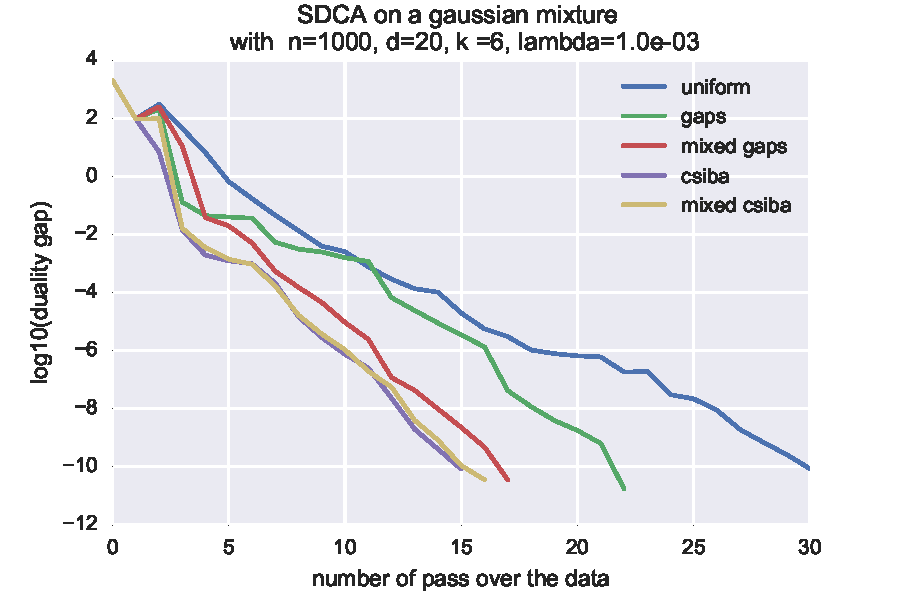
\includegraphics[width=.8\textwidth]{images/20170914_061831_gaussians_perf.pdf}
	\caption{Training curves for SDCA applied to the multinomial logistic regression on a dataset of a 1000 points drawn from 6 gaussians in dimension 20. Uniform indicates uniform sampling. Gaps indicates our proposed sampling scheme. Csiba indicates the scheme described in \ref{csiba}. Mixed gaps indicates that points are sampled uniformly half of the time, and proportionally to gaps the other half. Idem for mixed csiba.}
	\label{training gaussians}
\end{figure}


\paragraph{Covertype.}
We train a logistic regression model on the Covertype dataset \cite{blackard_comparative_1999} with SDCA.
The aim is to predict the kind of forest cover from geographic data. 
There are 7 kinds of forest cover.
We have $d'=54$ attributes (dimension of $x$).
We restrain the training set to ten thousand samples, and set $\lambda = 1/n$.
We observe the predicted linear rate.
The uniform sampling method is really not steep compared to the others. 
Once again, Csiba's scheme has the best result.
Its performance is very similar to the mixed schemes.
The method that samples purely based on duality gaps achieves a similar rate at first, but around $10^{-7}$ it nearly stops improving.

To sum it up, Csiba's method is most likely superior to ours.
A better empirical verification would require running this test on more datasets.
Nevertheless, a strong point of the duality gap approach is that it can be adapted effortlessly to the CRF model.

\begin{figure}[ht]
	\center
	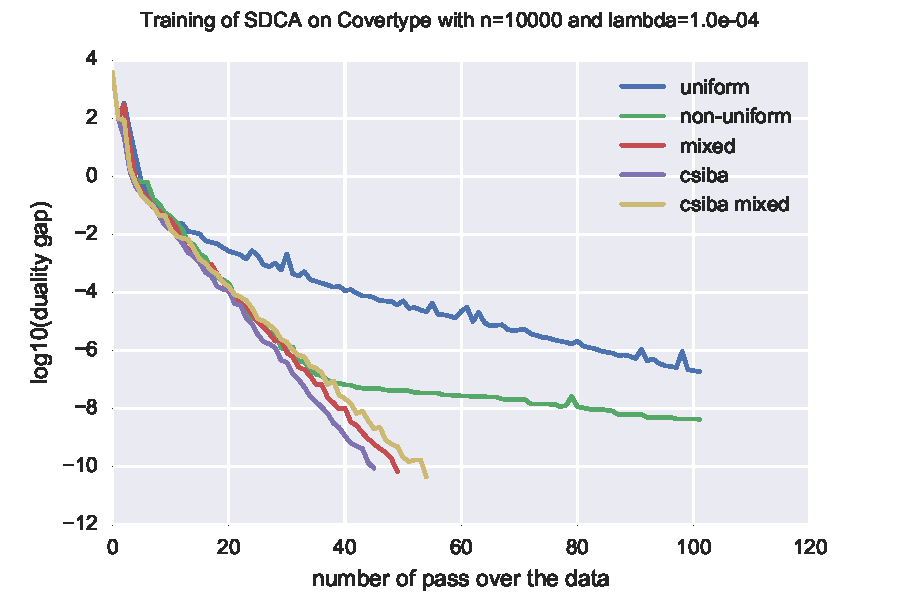
\includegraphics[width=.8\textwidth]{images/20170914_065817_covertype_perf.pdf}
	\caption{Training curves for SDCA applied to the multinomial logistic regression on the Covertype dataset. Uniform indicates uniform sampling. Gaps indicates our proposed sampling scheme. Csiba indicates the scheme described in \ref{csiba}. Mixed gaps indicates that points are sampled uniformly half of the time, and proportionally to gaps the other half. Idem for mixed csiba.}
	\label{training covertype}
\end{figure}

%%%%%%%%%%%%%%%%%%%%%%%%%%%%%%%%%%%%%%%%%%%%%%%%%%%%%%%
% CRF 
%%%%%%%%%%%%%%%%%%%%%%%%%%%%%%%%%%%%%%%%%%%%%%%%%%%%%%%
\clearpage
\section{Conditional Random Fields}

\subsection{Structured Prediction}

\paragraph{What is it?}
Structured prediction is a category of multi-class classification problems.
The particularity is that we have information about the structure of the classes.
For instance we would like to identify a word of length T from T images of letters, and we know that there is a chain structure on these letters (OCR dataset introduced in \cite{taskar_max-margin_2004}).
Or we could parse sentences and we know that there is a natural tree structure defined by the grammar.
Another typical instance is semantic segmentation in images : we know a priori that boundaries between objects should be sharp and that objects are usually connected areas.
We keep the same notations as before.
The difference is that now, for an input x, the label y will live in $\Y_x$ that depends on x.
For instance, in OCR the word we predict will have as many letters as we have images.
In semantic segmentation, the label will be an image of the same size as the input image, where the value of each pixel denotes the class of this pixel. 

\paragraph{Motivation.}
Compared to standard multi-class classification, we need to exploit the structure because the output space $\Y_x$ has a size that is typically exponential in the size of the input x.
Even for prediction, a brute force approach listing the probabilities class by class and taking the max is intractable.
The structure generally allows us to explore the space of classes in a clever way, to compute the mode of this distribution or the marginal probabilities on some part of the structure.
We call the algorithm that returns the mode the \textit{max oracle} and the one that returns the marginals the \textit{marginalization oracle}.
They are black boxes for the optimization algorithm, hence the name oracle.
They generally take time.
The performance of a structured prediction algorithm is generally measured by the number of oracle calls.
In reality, marginalization oracle are often slower than maximization oracle, and there are a number of operations besides these oracles.
However the number of oracle call is a simple and relevant estimation of the overall complexity.

\paragraph{What kind of structure?}
We consider an undirected graph $G=(V,E)$.
We denote $\mathcal{C}$ the set of cliques of G.
For a given label $y$ and a subset of vertices $s \subseteq V$, we denote $y_c$ the part of $y$ supported by these vertices.
We make the assumption that the feature extractor is separable over the cliques of that graph.
\begin{equation}
	F(x, y) =  \sum_{c\in \mathcal{C}} F_c(x, y_c)
\end{equation}
where we have clique feature extractors $F_c$.
The direct consequence is that the distribution $p(. | x ; w)$ will be Markov with respect to G.
It can be written as a product of potentials defined over the cliques of G.
\begin{align*}
	p(y|x ; w)
	& = \frac{1}{Z(x)} \exp(w^TF(x, y)) \\
	& = \frac{1}{Z(x)} \exp( \sum_{c \in \mathcal{C}} w^T F_c(x, y_c))\\
	& = \frac{1}{Z(x)} \prod_{c \in \mathcal{C}} \exp(w^TF_c(x, y_c))
\end{align*}
For a given x, its label y can be seen as a random variable whose distribution respect the Markov Random Field G.
This is the formal meaning of "labels have a structure".


\paragraph{Objectives.}
We have the same maximum likelihood objective as in the unstructured case.
The dual problem is the same, and the duality gaps are the same.
The difference is that the dual variable, which is a concatenation of joint probabilities, is now too large to be manipulated.

\subsection{Marginalization}
The raw dual problem is intractable.
The variable $\alpha$ is a priori too big to fit in memory : for each data point, it stores a probability vector whose length is exponential in the size of this data point.
This is where the structure comes into play.

\paragraph{Marginals.}
We define the marginal of $\alpha_i$ on the clique $c \in \mathcal C_i$.
\begin{equation}
	\label{marginals definition}
	\mu_{i, c}(y_c) := \sum_{y'\in \Y_i | y_c' = y_{i, c}} \alpha_i(y')
\end{equation}
The transformation from $\alpha_i$ to $\mu_i$ is linear.
We define $\mu_i \in \prod_c \Delta_|c|$ the concatenation of all the clique marginal vectors for the sample i.
We write $M_i$ the marginalization operator for sample i.
It is a matrix of size $\sum_{c \in \mathcal C_i} |\Y_c| \times |\Y_i |$.
The line $(c, y_c)$ of $M_i$ has a one on the columns $y'$ so that $y_c'=y_c$, and zeros everywhere else.
The column $y$ of $M_i$ has $|\mathcal C|$ ones, located on the lines $(c, y_c)$.
The vectorial form of equation \ref{marginals definition} is:
\begin{equation*}
	\mu_i = M_i \alpha_i
\end{equation*}
We define a global $\mu$ the concatenation fo all the $\mu_i$.
The global marginalization operator $M$ is a block diagonal matrix whose i-th block is $M_i$.
\begin{equation}
	\label{marginals vectorial}
	\mu = M \alpha
\end{equation} 

\paragraph{Feature centroids.}
Because the features are separable, we can write the dual weights as a function of the marginals :
\begin{align*}
	\E_{y \sim \alpha_i}[\psi_i(y)]
   	&  = \sum_{c \in \mathcal C_i} \E_{y \sim \alpha_i}  [\psi_{i, c}(y_c)]  \\
   	&  = \sum_{c \in \mathcal C_i} \E_{y_c \sim \mu_{i, c}}  [\psi_{i, c}(y_c)] 
\end{align*}
As we have done with $\bm w(\alpha)$, we can write this with vectors..
Let  $B_i$ be the matrix of size $d \times  \sum_{c \in \mathcal C_i} |\Y_c|$, whose column $(c, y_c)$ is $\psi_{i, c}(y_c)$.
\begin{equation*}
	 \E_{\alpha_i}[\psi_i] = B_i \mu_i
\end{equation*}
The dual weights are defined in equation \ref{dual to primal} as function of the joints. We can now express them as a function of the marginals.
\begin{align*}
	\bm w (\alpha)
	& =\frac{1}{\lambda n} \sum_i \E_{y \sim \alpha_i}[\psi_i(y)] \\
	& = \frac{1}{\lambda n} \sum_i B_i \mu_i
\end{align*}
Let $B$ be the horizontal concatenation of all the $B_i$. We write the function that gives the dual weights from the marginals with a calligraphic $\mathcal W$.
\begin{equation}
	\label{marginals to primal}
	\mathcal W (\mu) := \frac{1}{\lambda n} B \mu
\end{equation}
\textit{Remark:} one can verify that more generally, $A=BM$.

\paragraph{Junction Tree.}
We assume that the graph $G=(V,E)$ has a junction tree $T=(\mathcal C_{max},\mathcal{S})$.
$\mathcal C_{max} \subset \mathcal C $ is the set of maximal cliques of G.
$\mathcal S$ is a set of separations (= intersection) of these cliques, that defines the tree $T$.
The direct consequence is that we can run message passing on the junction tree.
That means \textbf{we have a marginalization oracle} at hand : for any weight vector $w$ and data point $x$ we can infer the marginals $p_c(y_c |x ; w)$.
The second consequence is that \textbf{the joint probability $\alpha_i(y)$ can be written as a function of its marginals $\mu_{i, c}$}.
\begin{equation}
	\label{joint from marginals}
	\alpha(y) = \frac{\prod_{c\in\mathcal{C}_{max}} \mu_c(y_c)}{\prod_{s\in\mathcal{S}} \mu_s(y_s)}
\end{equation}
This formula make sense as long as the marginals on the maximal cliques are coherent, meaning that they agree about the values of the marginals on the separations.
Our algorithm will make sure that this coherence is preserved at each step.
Equation \ref{joint from marginals} allows us to translate the entropy and the Kullback-Leibler divergence of joint probabilities as functions of their marginals. We write these new functions with calligraphic letters.
\begin{align}
	\label{marginals entropy}
	\mathcal H (\mu) := H_{|\Y|} (\alpha) & = \sum_c H_{|c|}(\mu_c) - \sum_s H_{|s|}(\mu_s) \\
	\label{marginals divergence}
	\mathcal D (\mu||\mu') := D(\alpha||\alpha') & = \sum_c D(\mu_c||\mu_c') - \sum_s D(\mu_s||\mu_s')
\end{align}


\paragraph{Dual Objective.}
With equations \ref{marginals to primal} and \ref{marginals entropy} we can express the dual problem as a maximization over the marginals.
\begin{equation}
	\max_{\forall i \forall c, \mu_{i, c} \in \Delta_{|c|} } - \frac{\lambda}{2} \| \mathcal W(\mu)\|^2 + \frac{1}{n} \sum_i \mathcal H _ i(\mu)
\end{equation}
Equation \ref{marginals divergence} even allow us to compute duality gaps.
When we replace the joint $\alpha_i$ with the marginal $\mu_i$, we go from a size $|\Y_i|$, to a size $\mathcal U_i := \sum_{c \in \mathcal C_i} |\Y_c|$.
If each component of y can take $K=26$ values, and the typical word length is 7, as in the OCR dataset, then we go from $K^T \sim 10^{10}$ to $\sum_{c \in \mathcal C_i} K^{|c|} \sim 10^3$.
We replace a problem that is intractable with a problem that is tractable.

\subsection{Stochastic Dual Coordinate Ascent}
SDCA will now update the marginal probabilities $\mu_i$ instead of the $\alpha_i$. 
There are few consequences to this marginalization.
The main one is that we have to call a marginalization oracle to get the marginals from the weights.
More generally, every function of the joint should be replaced by its marginals counterpart. 

\begin{algorithm}[ht]
    \caption{SDCA for CRF}%
    \label{sdca for crf}
\begin{algorithmic}
        %
        \STATE Let $\forall i, c, \mu_{i, c}^{(0)} := \frac{1}{|c|}$ and $w^{(0)} := \frac{1}{\lambda n} B \mu^{(0)} $
        \STATE Let $\forall i g_i = 1$ (optional)
        %
       \FOR{$k=0\dots K$}
                \STATE Pick $i$ at random in $\{1,\ldots,n\}$ (optionally, proportional to $g_i$)
                \STATE Compute $\forall c, \mu_{i, c}' (y_c) := p(y_c|x; w^{(k)})$ (marginalization oracle)
                %
                \STATE Let $g_i = \mathcal D(\mu_i || \mu_i')$ (optional)
                %
                \STATE Let $d_i = \mu_i' - \mu_i^{(k)}$ (ascent direction)
                \STATE Let $v_i = \frac{1}{\lambda} B_i d_i $ (primal direction)
                \STATE Solve $\gamma^* = \argmax_{\gamma \in [0,1]} \mathcal H_i(\mu_i^{(k)} + \gamma d_i) - \frac{\lambda n}{2} \| w^{(k)} + \frac{\gamma}{n} v_i \|^2$ (Line Search)
                %
               \STATE Update $\mu_i^{(k+1)} := \mu_i^{(k)} + \gamma^* d_i$
               \STATE Update $w^{(k+1)} := w^{(k)} + \frac{\gamma^*}{n} v_i $
        \ENDFOR
\end{algorithmic}
\end{algorithm}

\paragraph{Initialization.}
Another consequence is that we can no longer initialize the variable randomly. 
The marginals have to be coherent on the separations of the junction tree.
A solution would be to initialize the weights randomly, and then to do a full batch marginalization.
This is the same cost as running SDCA over the whole dataset once.
A simpler and more economical solution is probably to initialize the marginals to the uniform distributions.
That means starting with the highest entropy possible and with a very low data fitting.

Another solution would be to initialize the marginals with the empirical marginals.
That means starting with a dual score equal to zero : lowest entropy and highest data fitting.
The problem is that the gradient of the entropy is not defined on the boundary of the simplex.
Our algorithm is meant to evolve in the interior of the simplex. 
This is in contrast with the Structured SVM setting where the optimal probabilities are sparse \cite{lacoste-julien_block-coordinate_2012}.
They lie on borders of the simplex.
The uniform marginals is central to the simplex.
It is also the probability given by the weight vector zero : $\mu_{\textrm{uniform}} = p(. |x ; w=0)$.
The weight vector zero is also a sensible initialization when one look at the primal problem.

Note that the computation of $w^{(0)}$ can usually be done very efficiently for a uniform marginal.
It does not suffer a $O(n d \mathcal U)$ complexity.
For the empirical marginals, it is even simpler: $w^{(0)}=0$.

\paragraph{Line Search:} 
It is mostly the same as the first line search.
We just have to consider the right functions of the marginals.
The marginals over the separations $\mu_{i, s}$ and $d_{i, s}$ are computed once and for all at the beginning of the line search.
The quadratic and the linear term as well.


\begin{align*}
	f(\gamma)
	& = \mathcal H_i(\mu_i^{(k)} + \gamma d_i) 
	- \frac{\lambda n}{2} \| w^{(k)} + \frac{\gamma}{n} v_i \|^2 
	\\
	& =  \sum_c H_{|c|}(\mu_c + \gamma d_{i, c}) 
	- \sum_s H_{|s|}(\mu_s + \gamma d_{i, s}) 
	- \frac{\lambda n}{2} \| w^{(k)}\|^2 
	- \gamma \lambda  \langle w^{(k)} , v_i \rangle 
	- \gamma^2 \frac{\lambda}{2n} \|v_i \|^2 
	\\
	f'(\gamma) & =  - \sum_c \langle d_{i, c}, \log(\mu_c + \gamma d_{i, c}) \rangle 
	+ \sum_s \langle d_{i, s} , \log(\mu_s + \gamma d_{i, s}) \rangle 
	- \lambda  \langle w^{(k)} , v_i \rangle 
	- \gamma \frac{\lambda}{n} \|v_i \|^2 
	\\
	f''(\gamma) & = - \sum_c \sum_{y_c} \frac{d_{i, c}(y_c)^2 }{ \mu_c(y_c) + \gamma d_{i, c}(y_c) }
	+ \sum_s \sum_{y_s} \frac{d_{i, s}(y_s)^2 }{ \mu_s(y_s) + \gamma d_{i, s}(y_s) }
	- \frac{\lambda}{n} \|v_i \|^2 
\end{align*}

\paragraph{Complexity:}
SDCA performs one and only one marginalization oracle call per step.
This is its main advantage over its counter part, Stochastic Average Gradient with Non-Uniform Sampling \cite{schmidt_non-uniform_2015}.
In NUS-SAG, the non-uniform sampling scheme depends on estimators of the Lipschitz constants.
These estimators are also used to set the step size.
They are found via a line search for which each function evaluation requires an oracle call.
Some heuristics are used to spend less time in these line search.
In comparison, SDCA performs exact line search at each step, with only one oracle call.
We write $\mathcal U_i = \sum_c |\Y_c|$. The complexity of the other parts of the algorithm are:
\begin{itemize}
	\item Non-uniform sampling $O(\log n)$.
	\item Duality gap estimation $O(\mathcal U_i)$
	\item Dual ascent direction $O(\mathcal U_i)$
	\item Primal descent direction $O(d \ \mathcal U_i)$, although there are ways to make it faster, depending on the structure of the features.
	\item Function estimation in the Line Search $O(\mathcal U_i)$
\end{itemize}

In terms of memory, SDCA has the same complexity as SAG. 
Both methods need to store the marginals.
For a general pairwise graphical model with V vertices, E edges, and K class per nodes, this is a total complexity of $O(n(VK + EK^2))$.

\subsection{Results on OCR}

We implemented the SDCA method as well as all the subroutines to train a CRF on the OCR dataset.
We implemented everything in Python with Numpy.
The oracles that we need are the sum-product algorithm and the max-product algorithm on a chain.
They both are dynamic programming algorithm that can be implemented in relatively few lines.
The features we used are described in appendix I.1 of \cite{osokin_minding_2016}.

There are two complicated objects in the algorithm \ref{sdca for crf} : the marginals and the features.
We implement both of them as classes, so that applying SDCA on a  new dataset with a sequential structure will just require to implement these classes again.

The algorithm is not working yet.
There is most likely a bug.
We provide preliminary results to show what works and what does not, and more importantly to give some insights about the algorithm itself. 
For the reference, we include the figure \ref{schmidt's curves} drawn from \cite{schmidt_non-uniform_2015}.
In this figure, a number of methods are compared on the OCR dataset.
The best one is SAG-NUS* : stochastic average gradient with a line search and a mixed uniform -- non-uniform sampling scheme.
SAG-NUS* reaches a sub-optimality of $10^{-4}$ on the primal in about a 100 iterations.

\begin{figure}[ht]
	\center
	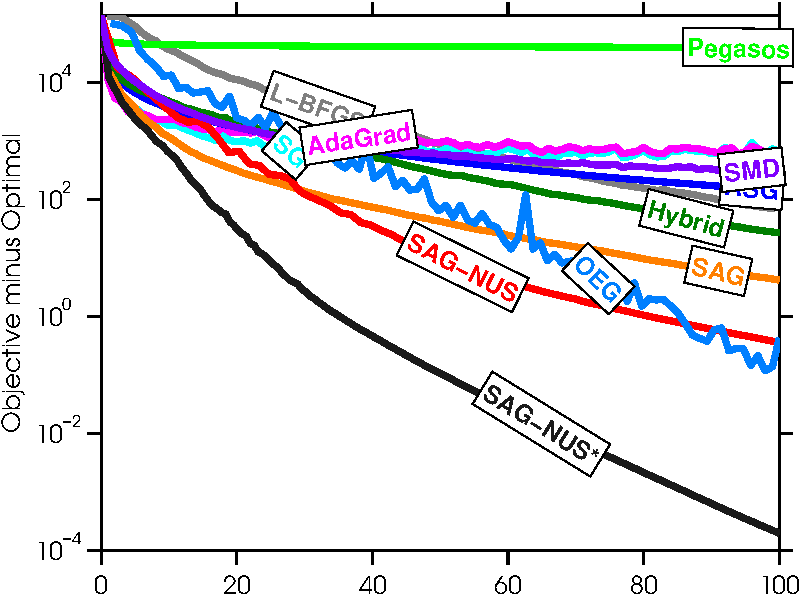
\includegraphics[width=.5\textwidth]{images/ocr2_train_passes.pdf}
	\caption{Training curves for various optimization algorithms on the OCR dataset. The x axis is the number of epochs, while the y axis is the primal suboptimality.}
	\label{schmidt's curves}
\end{figure}


Figure \ref{training crf} shows the evolution of the duality gap on a subset  of  the OCR dataset  of size $n=626$, for different values of $\lambda$.
When $\lambda=1$ (very large), the duality gap decreases very fast towards $10^{-2.5}$, at which it stops.
When $\lambda$ gets to smaller, more reasonable values, the algorithm gradually stop converging, and even worse, it starts increasing the duality gap.

\begin{figure}[ht]
    \centering
    \begin{subfigure}[t]{\textwidth}
        \centering
        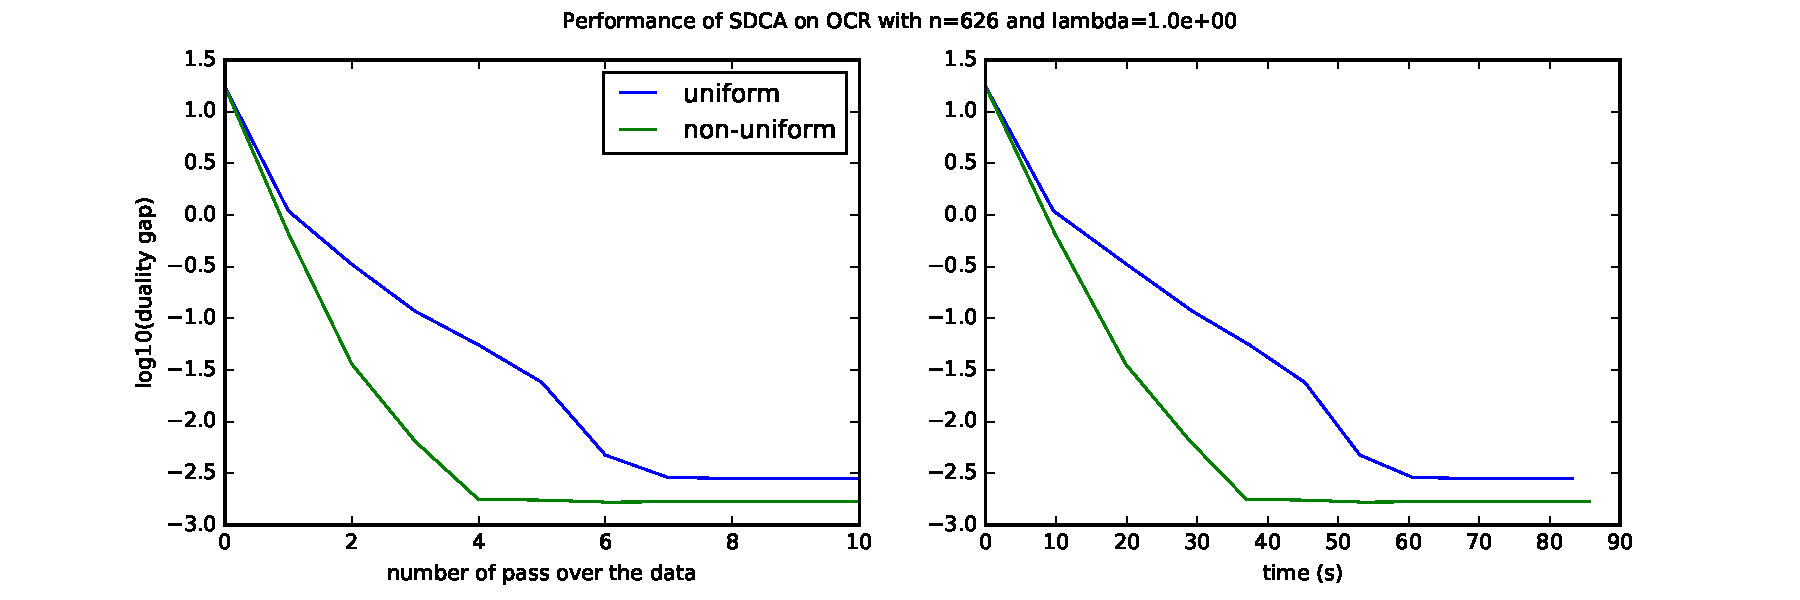
\includegraphics[width=\textwidth]{images/20170914_040237_ocr_perf.pdf}
    \end{subfigure}

    \begin{subfigure}[t]{\textwidth}
        \centering
        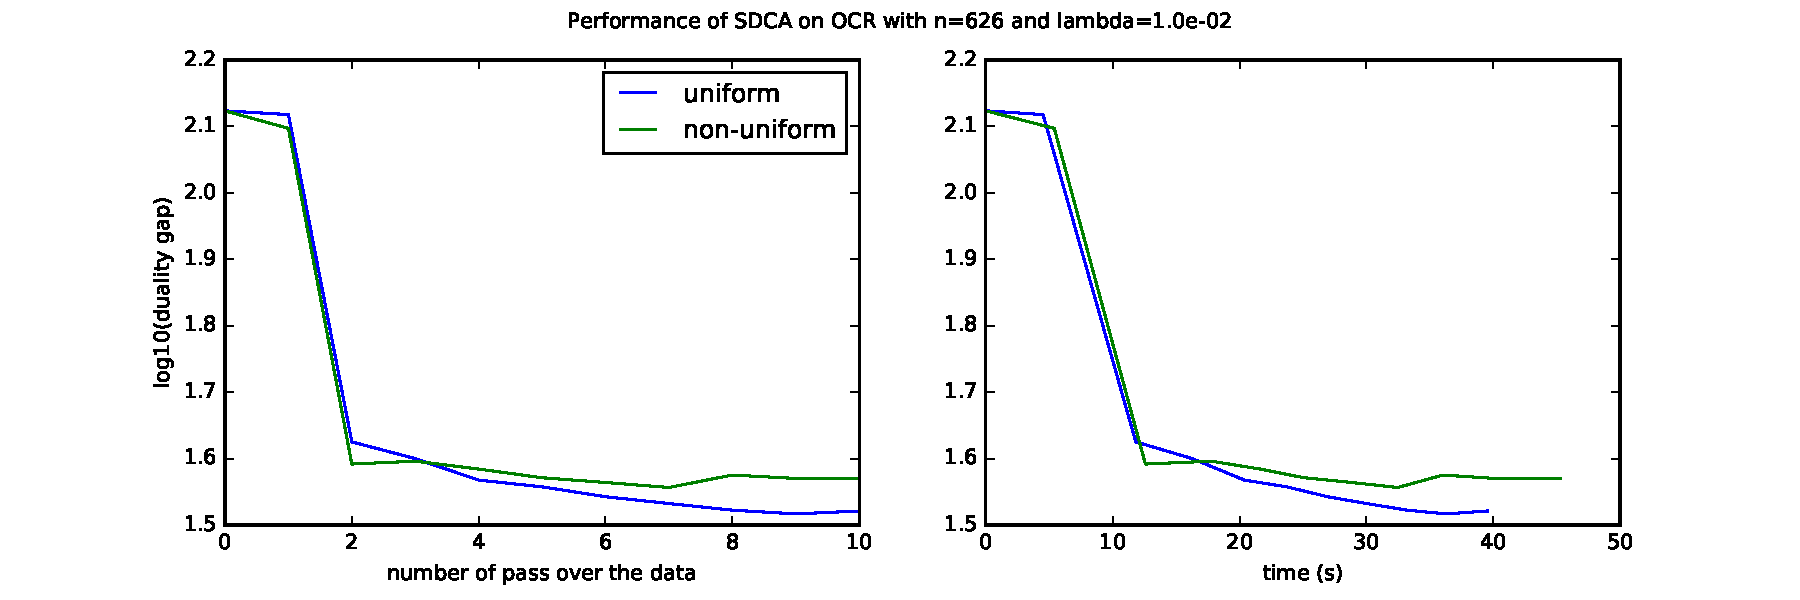
\includegraphics[width=\textwidth]{images/20170914_041643_ocr_perf.pdf}
    \end{subfigure}

    \begin{subfigure}[t]{\textwidth}
        \centering
        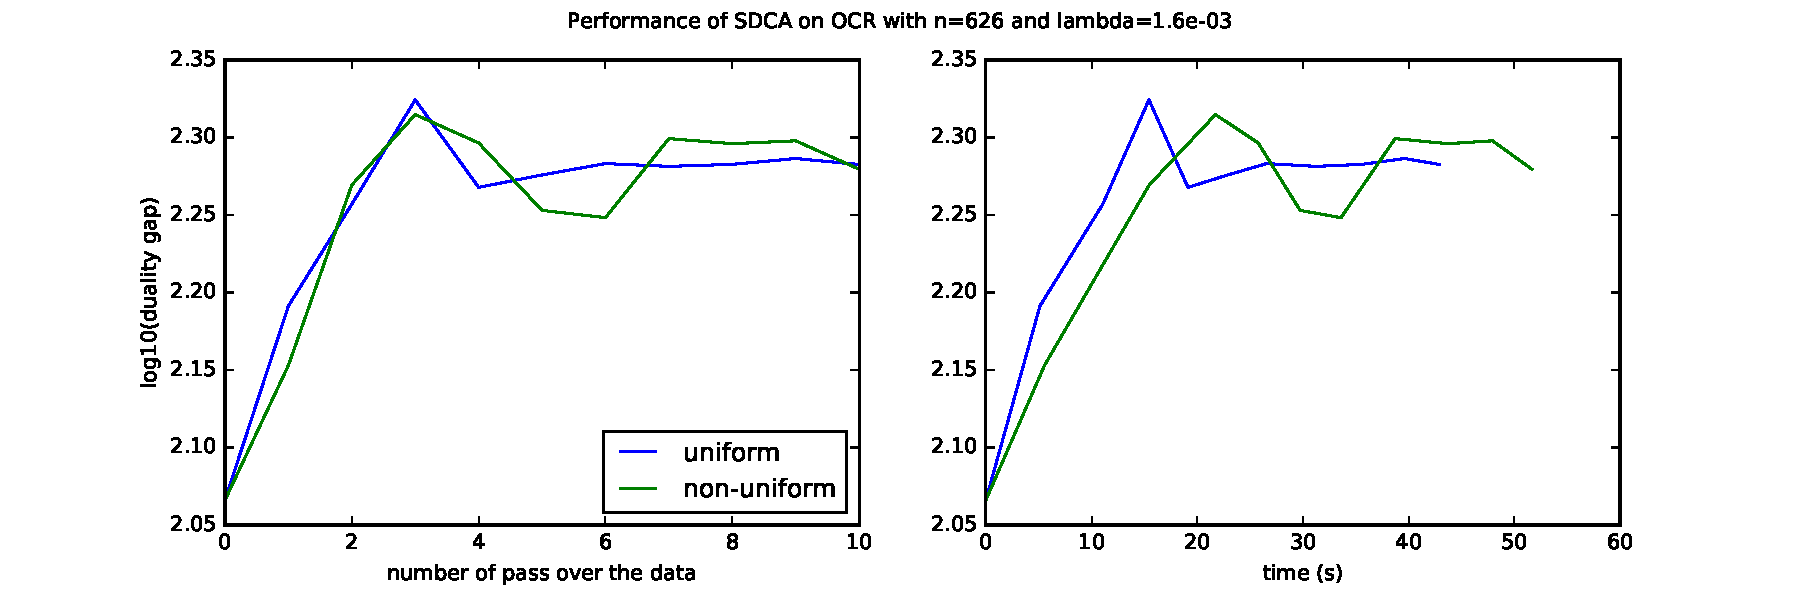
\includegraphics[width=\textwidth]{images/20170914_040715_ocr_perf.pdf}
    \end{subfigure}
    \caption{Training curve of SDCA on OCR for various parameters $\lambda$.}
    \label{training crf}
\end{figure}


In figure \ref{ocr annexes}, we look at the evolution of some variables to get some insights on the behaviour of SDCA. 
On the top, there is the norm of the primal descent direction.
Second is the inner product between the weight vector and the primal descent direction.
A negative inner product is a good thing since we want to minimize the norm of the weight vector.
This is especially true at the beginning because we initialize SDCA with the uniform distribution.
From there the entropy can only decrease to let the weight norm decrease as well.
The plots show that indeed the inner product is mostly negative before oscillating around the zero line. 
These two first variables are used in the definition of the line search.
Both of them should converge towards zero.
The norm of the ascent direction does not for small values of $\lambda$.

The third line of plots represent the evolution of the step size.
In every instance, they tend to be high and close to 1 at the beginning.
After a few pass, they tend to be mostly zero.
In total, about 70\% of the samples we pick are useless (step size = 0).

The fourth line is the evolution of the dual score.
This is the score that we are directly optimizing in SDCA.
It increases as we expect, and it looks converging.
Yet for the two small values of $\lambda$, it remains negative.
It performs worse than the empirical distribution (score equal zero).

Finally the fifth line is the estimate of the duality gap that we get by taking the mean of the (stale) individual duality gaps.
We observe a jump after each epoch.
That corresponds to the full batch computation of the duality gap, resetting the estimate to its true value.
If the algorithm was running normally, we would do that operation only every five or ten epochs.

\begin{figure}[ht]
    \centering
    \begin{subfigure}[t]{0.3\textwidth}
        \centering
        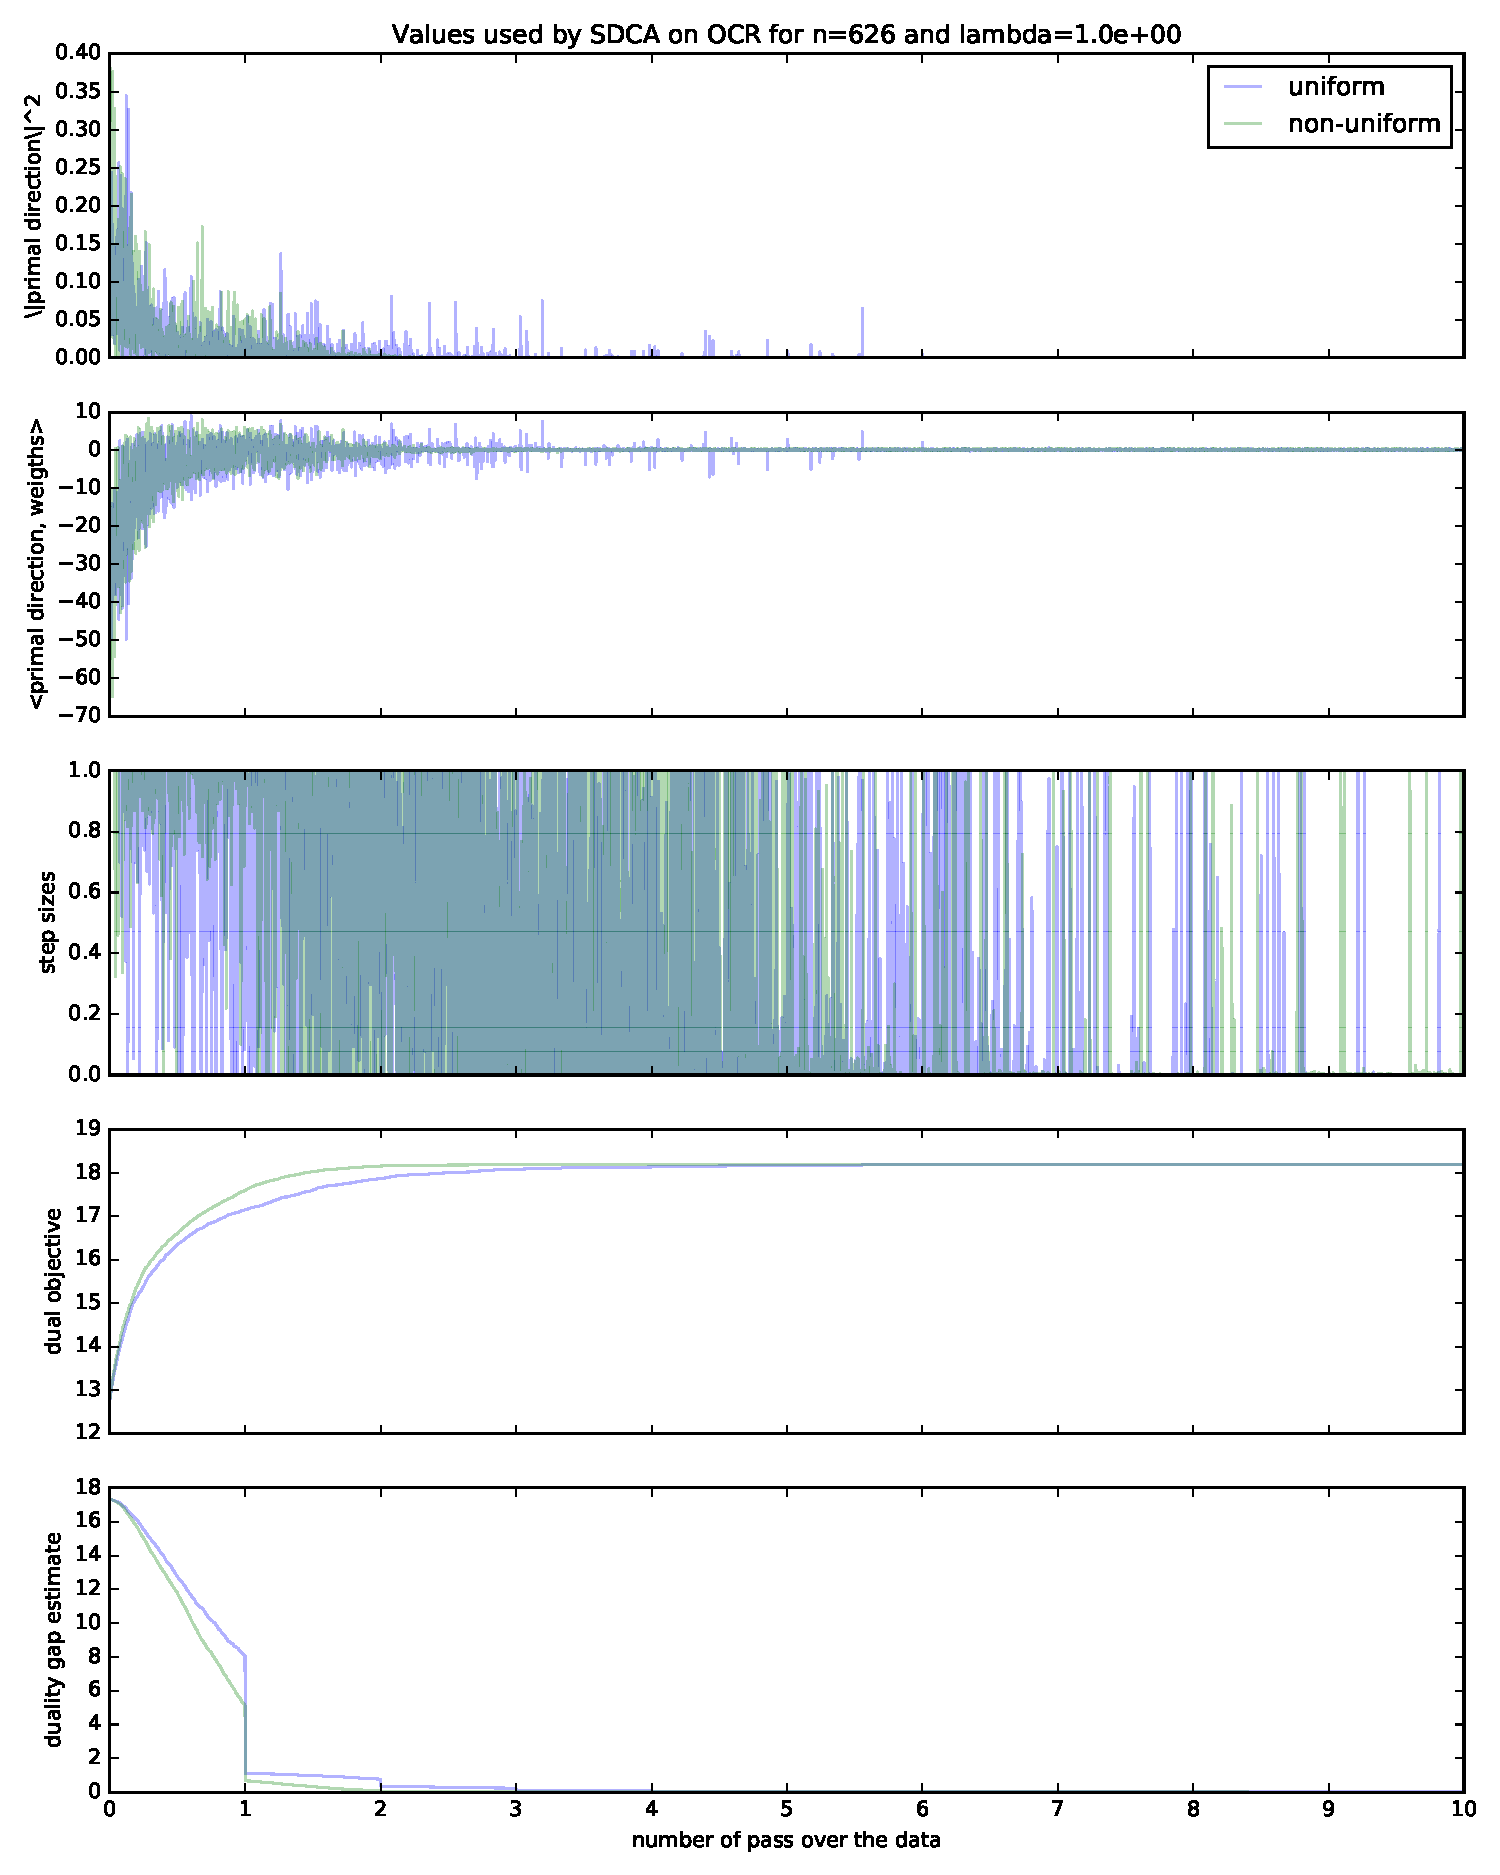
\includegraphics[width=\textwidth]{images/20170914_040249_ocr_annex.pdf}
    \end{subfigure}
    ~
    \begin{subfigure}[t]{0.3\textwidth}
        \centering
        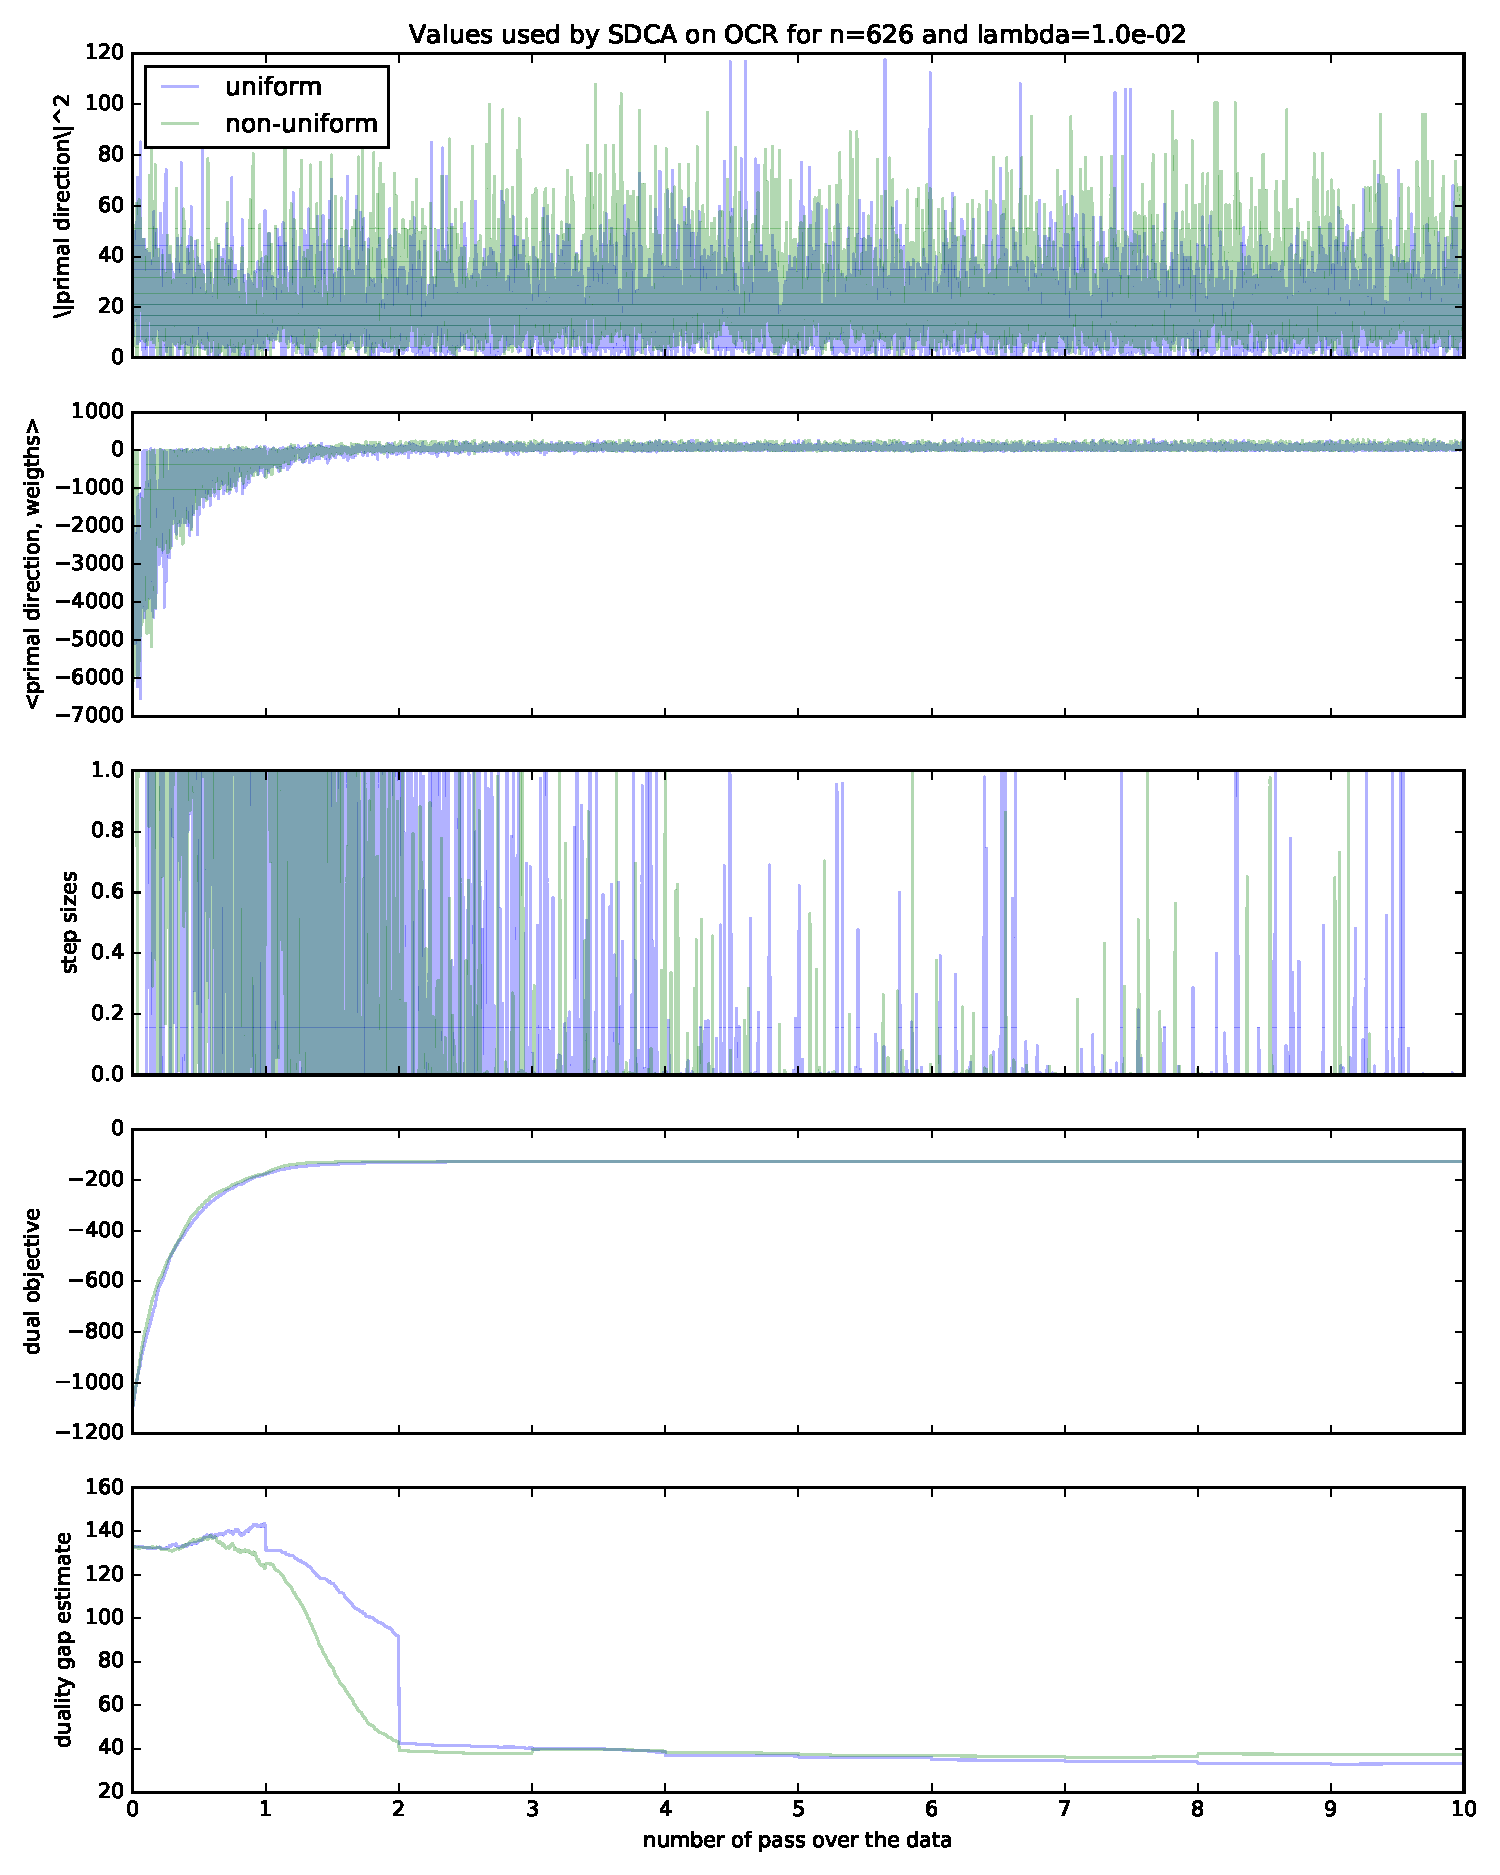
\includegraphics[width=\textwidth]{images/20170914_041645_ocr_annex.pdf}
    \end{subfigure}
    ~
    \begin{subfigure}[t]{0.3\textwidth}
        \centering
        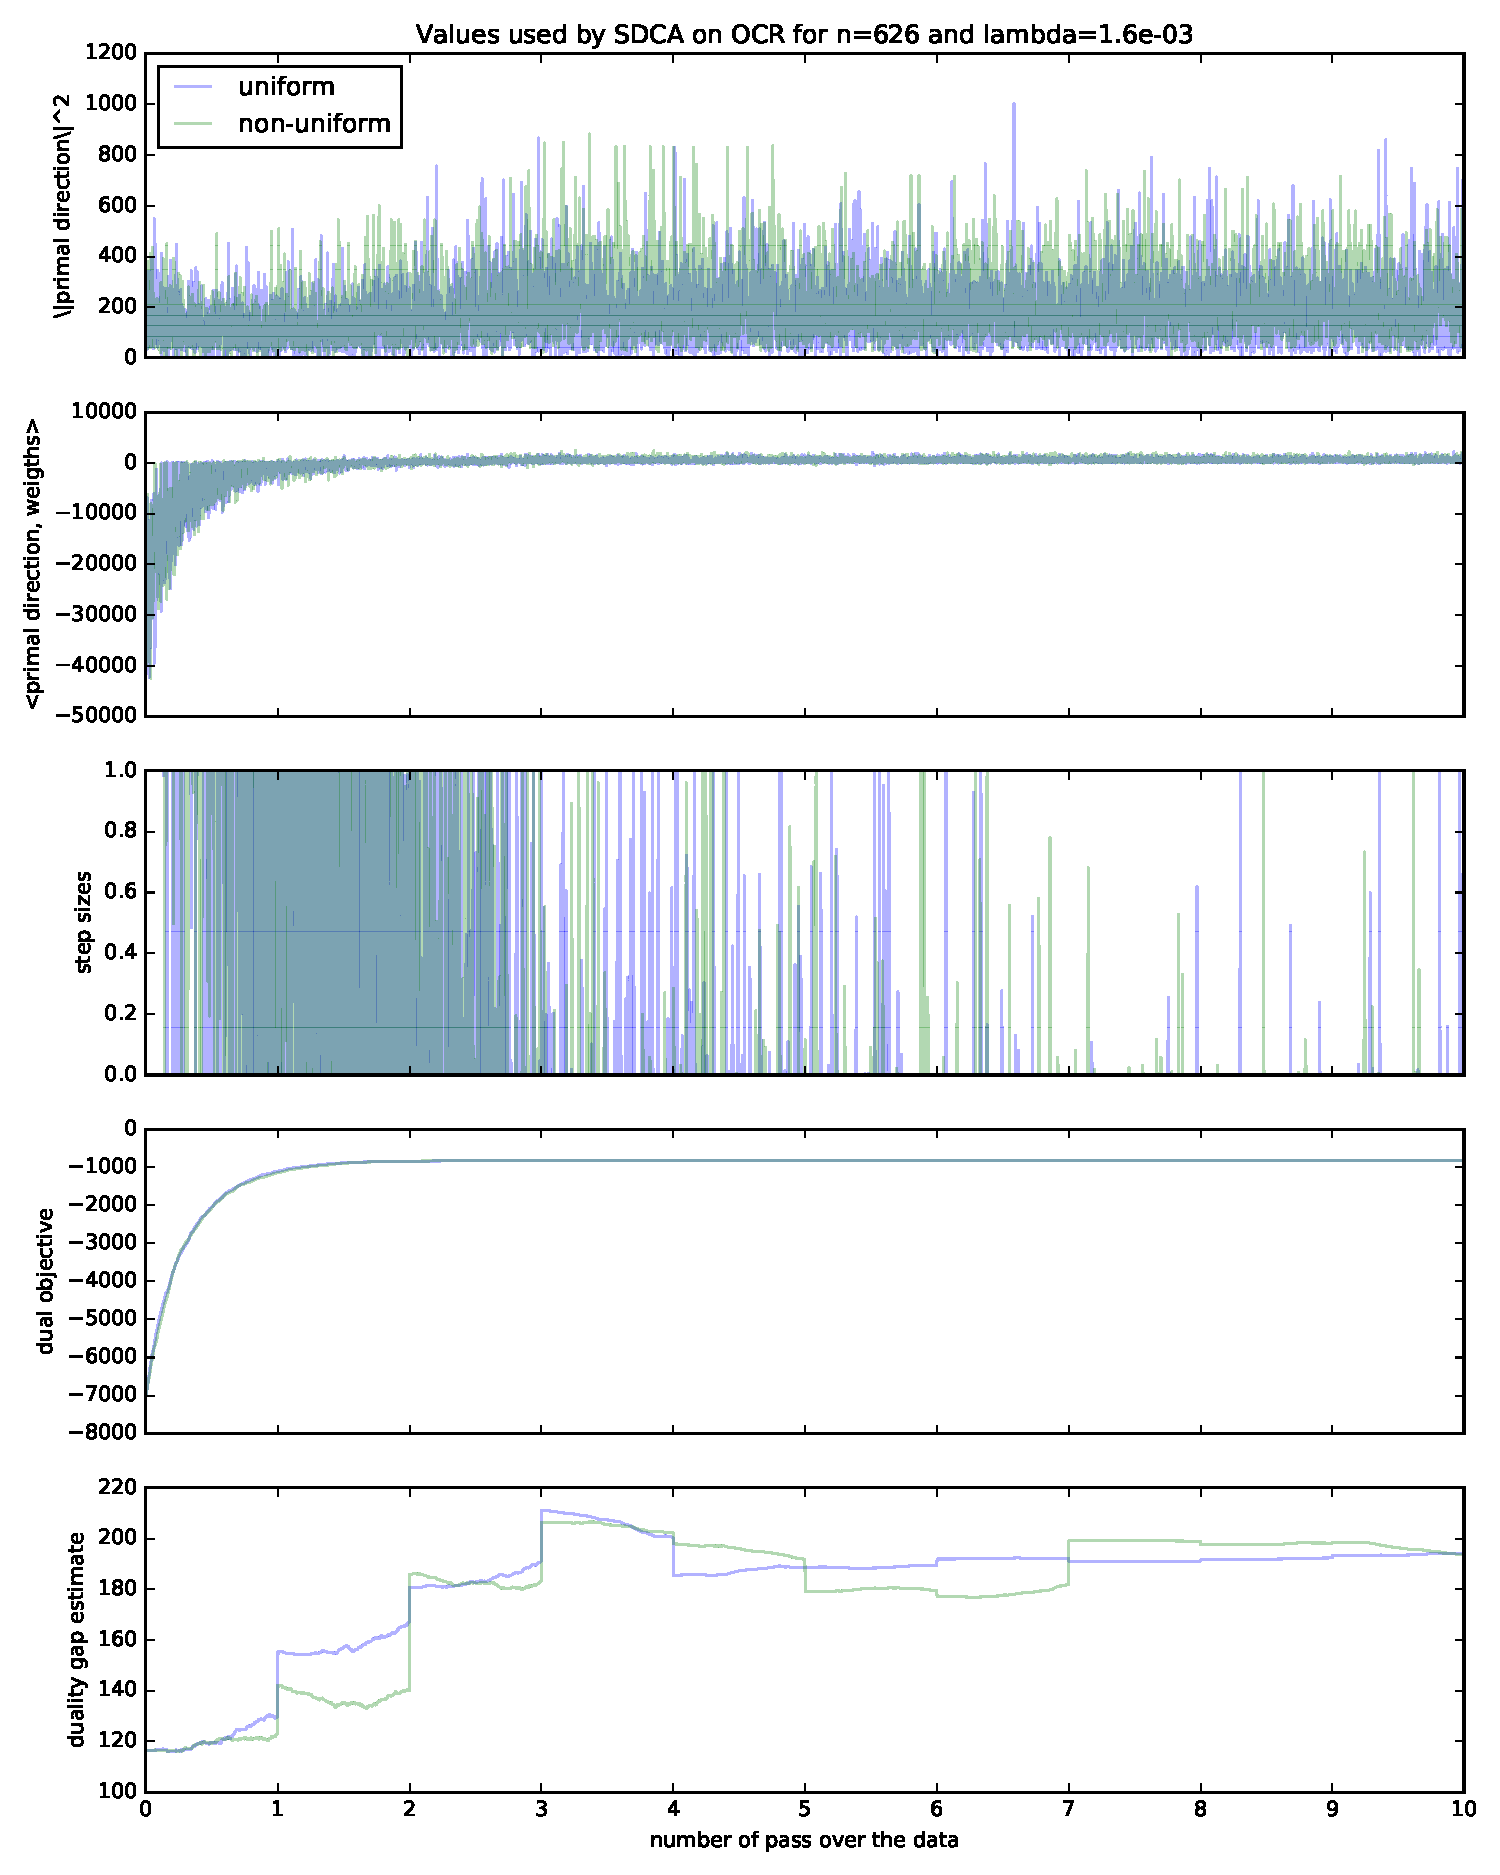
\includegraphics[width=\textwidth]{images/20170914_040717_ocr_annex}
    \end{subfigure}
    \caption{Some values of interest tracked along the run of SDCA.}
	\label{ocr annexes}
\end{figure}


\begin{figure}[ht]
    \centering
    \begin{subfigure}[t]{0.3\textwidth}
        \centering
        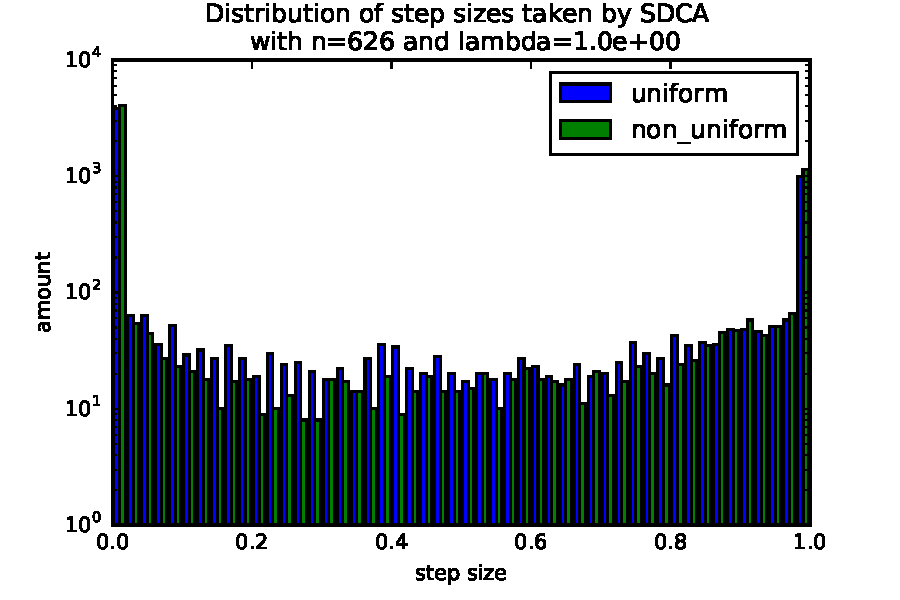
\includegraphics[width=\textwidth]{images/20170914_040255_ocr_stepdistrib.pdf}
    \end{subfigure}
    ~
    \begin{subfigure}[t]{0.3\textwidth}
        \centering
        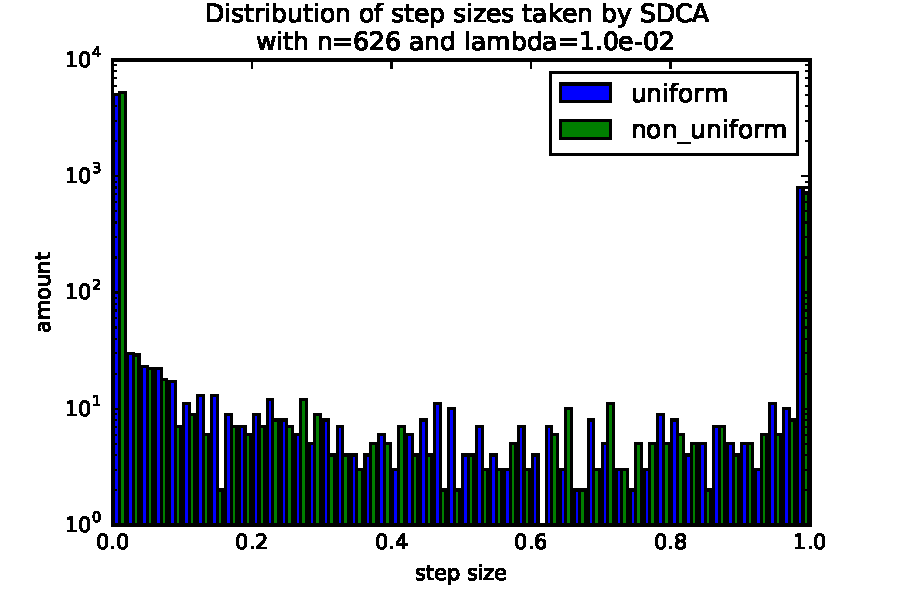
\includegraphics[width=\textwidth]{images/20170914_041649_ocr_stepdistrib.pdf}
    \end{subfigure}
    ~
    \begin{subfigure}[t]{0.3\textwidth}
        \centering
        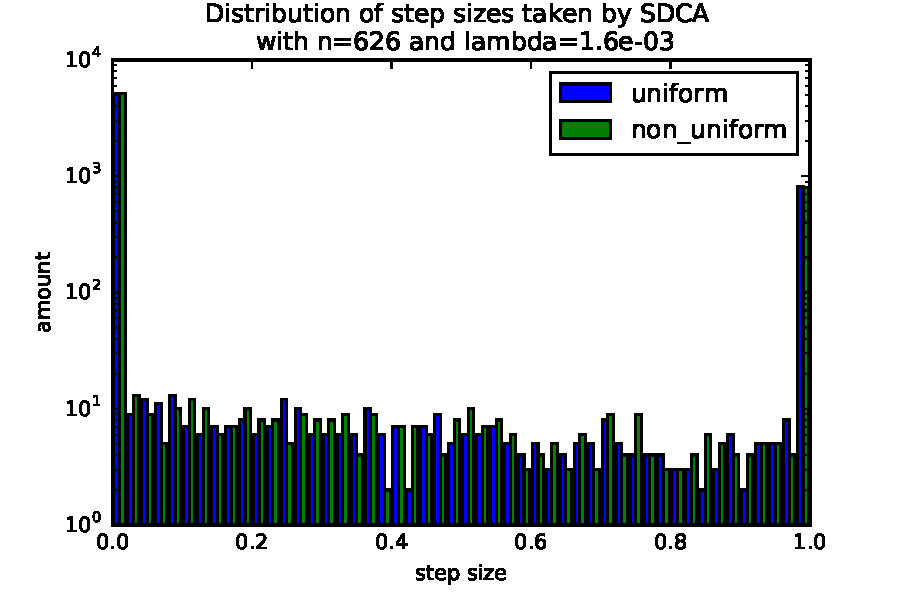
\includegraphics[width=\textwidth]{images/20170914_040720_ocr_stepdistrib.pdf}
    \end{subfigure}
    \caption{Distributions of step sizes taken by SDCA. The y axis is a log-scale. A large majority of steps are either taken with full size 1, either not taken at all. When the algorithm works better, with $\lambda$ large, there are more intermediate step sizes.}
	\label{ocr step sizes}
\end{figure}

\begin{figure}[ht]
    \centering
    \begin{subfigure}[t]{0.3\textwidth}
        \centering
        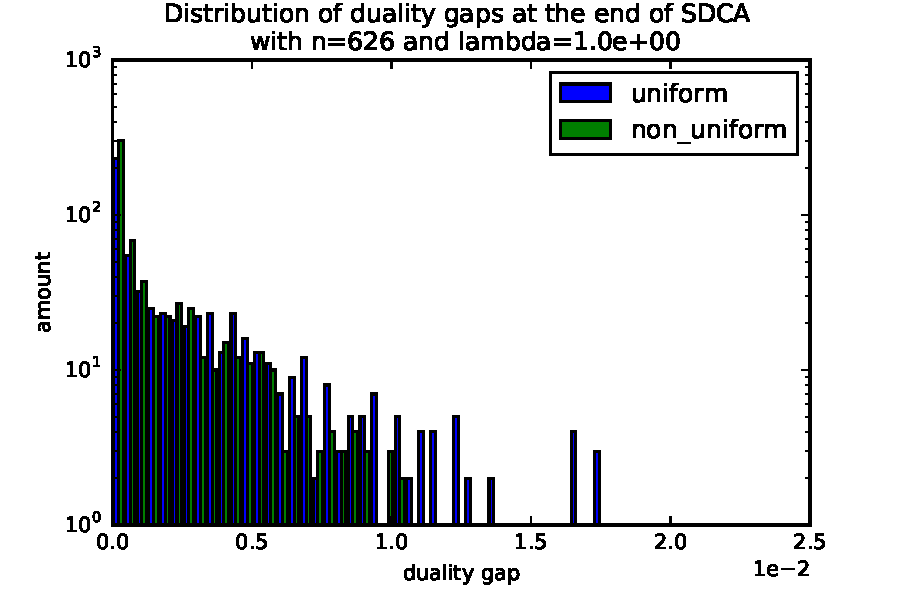
\includegraphics[width=\textwidth]{images/20170914_040308_ocr_optdualgaps.pdf}
    \end{subfigure}
    ~
    \begin{subfigure}[t]{0.3\textwidth}
        \centering
        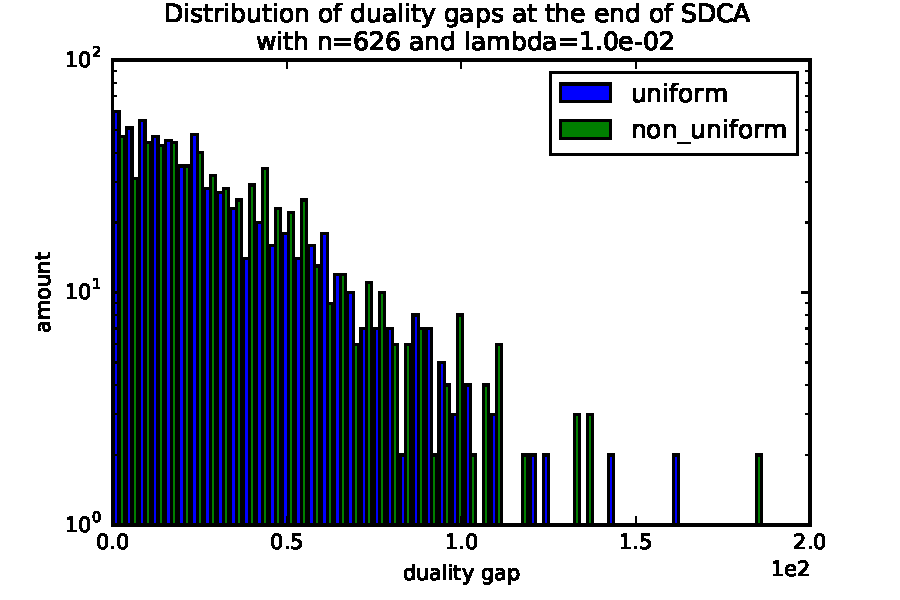
\includegraphics[width=\textwidth]{images/20170914_041703_ocr_optdualgaps.pdf}
    \end{subfigure}
    ~
    \begin{subfigure}[t]{0.3\textwidth}
        \centering
        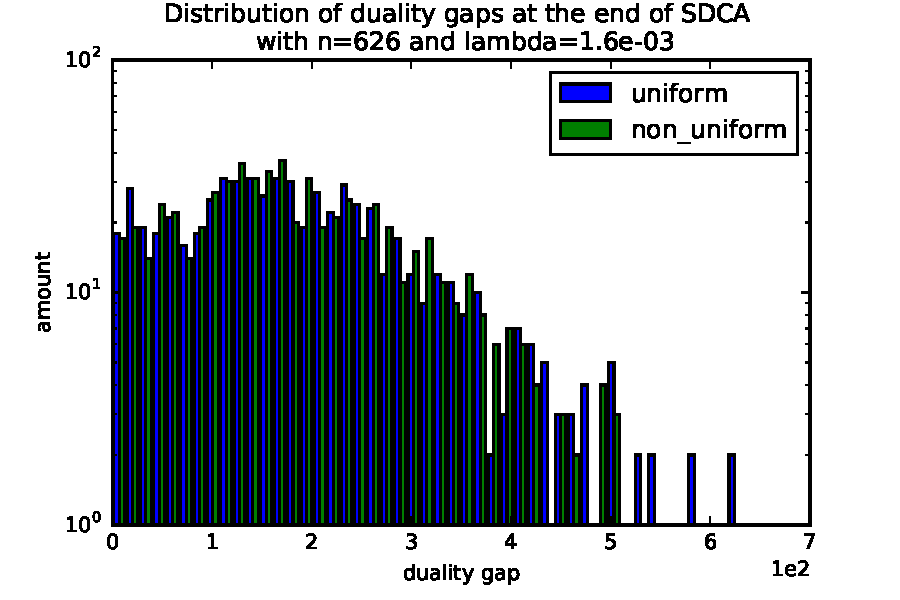
\includegraphics[width=\textwidth]{images/20170914_040725_ocr_optdualgaps.pdf}
    \end{subfigure}
    \caption{Distribution of individual duality gaps after the run of SDCA.}
	\label{ocr duality gaps}
\end{figure}


\section*{Conclusion}

SDCA is applicable to train CRF models. 
We still lack experimental evidences of its efficiency.
Chances are that there exist a domain for which SDCA is more efficient than SAG, as illustrated by the complexity analysis.
This project is still going on at the MILA.


\bibliographystyle{plain}
\bibliography{optimization.bib}

\end{document}